%!TEX program = xelatex
\documentclass[cn,normal,11pt,black]{elegantnote}
\usepackage{graphicx}
\usepackage{multirow}
\usepackage{lscape}
\usepackage{amsmath}
\usepackage{amsfonts}
\usepackage{amsthm}


\title{暨大经院高宏通关笔记}
\author{胡弘宇
\thanks{本学期我在王贤彬老师处听课,感谢同门林萍容提供的戴天仕老师的课堂笔记。
需要指出的是,王老师侧重教材,会按照教材的逻辑一步步推导,同时阐述背后的经济学逻辑,有助于模型的理解。
戴老师则将每个章节的内容直接提炼为统一的数理模型,只要把握住了模型一致的内在逻辑,做题就很顺手。
因此,一定程度上本文可视作王老师与戴老师课堂内容的综合版。
感谢以下同学指出之前版本存在的严重错误:区经黄莹欣、国贸汤城建、政经吴若楠、财政鲁浚豪等。}}
\institute{国贸系2018级}
\version{2.20}
\date{\today}

\begin{document}
\maketitle
\setlist[itemize]{label=$\circ$}

这份笔记最初是我为自己在最后一天清关背诵而写的,
分享出去后收到了一些反馈,发现其“外部性”很高,
故有此后续版本的更新。
希望能有效减少大家的信息搜集与整理成本,提高复习效率!
需要指出的是,这份笔记以各模型的定义、推导、计算逻辑为主要内容,
删去了教材中不少细节部分,更适合后期强化复习时使用。
\footnote{课堂使用教材:\\
David Romer, Advanced Macroeconomics, forth Edition (McGraw-Hill, 2011)\\
Daron Acemoglu, Introduction to modern economic growth (Princeton University Press, 2009) \\
课外推荐教材: \\
    Robert J. Barro and Xavier Sala-i-Martin, Economic Growth.
    (The MIT Press, 2003) \\
    Philippe Aghion and Peter Howitt, The Economics of Growth.
    (The MIT Press, 2008) \\
    Michael Wickens, Macroeconomic Theory: A Dynamic General Equilibrium Approach.
    (Princeton University Press, 2012)
}
我已将之作为个人项目上传到我的~\href{https://github.com/jun3970/MacroNote.JNU}{github主页},
\text{https://github.com/jun3970},方便大家协作编辑与下载。  


\renewcommand{\abstractname}{内容提要}
\begin{abstract}
本学期宏观课程内容由 Romer的 \textit{Advanced Macroeconomics} 第1、2章
和 Acemoglu 的 \textit{Introduction to Modern Economic Growth} 第2、11、12、13、14章组成。
包含六个模型:经典Solow模型,Ramsey-Cass-Koopmans模型(RCK),
Diamond overlapping-generations模型(OLG),AK模型(Solow版、Ramsey版、Romer版),
以及种类扩张模型和质量阶梯模型。
总结所学内容可分为以下四点,
\begin{itemize}
    \item 寻找平衡增长路径(BGP),以及BGP上的消费动态路径$\dot{c}_t/c_t$和资本动态路径$\dot{k}_t$。
    \item 计算均衡消费量$c^*$和资本存量$k^*$,有时还涉及储蓄率$s_t$
    \item 福利分析,即对比市场均衡$g^*_c$与社会计划下的$g^s_c$
    \item 政策效应,内容大多集中在征税或补贴,包括对资本收益、工资、销售收入以及研发投入等,稍微复杂一点的是对厂商定价做出限定。
\end{itemize}
\end{abstract}


\newpage
\section{预备知识}
\begin{theorem}[变量的增长率]
    宏观经济学最重要的议题之一是经济增长,分析这类问题要求我们简洁刻画模型中变量的增长率。
    不断加减再做除的计算过程麻烦且无趣,
    现有一巧妙方法——变量增长率等于其自然对数关于时间$t$的一阶导数。
    证明如下,
    \begin{equation*}
        \frac{d \ln X_t}{d t} = \frac{d \ln X_t}{d \ X_t} \; \frac{d X_t}{d \ t} 
                                = \frac{\dot{X}_t}{X_t} .
    \end{equation*}
    其中,变量顶部加点表示对该变量关于时间$t$求一阶导,即$\dot{X}_t =  d X_t / d t$。

\end{theorem}

\begin{proposition}[增长率的基本性质]
    令$\dot{X}_t/X_t = \omega$,
    易证此时有$X_t = X_0 \ e^{\omega t}$。此外
    \begin{itemize}
        \item 两个变量之积的增长率等于其各自增长率之和
        \item 两个变量之比的增长率等于其各自增长率之差
        \item 若$y_t=k_t^\alpha$, 则$\dot{y_t}/y_t = \alpha (\dot{k_t}/k_t)$
    \end{itemize}
\end{proposition}

\begin{theorem}[Hamiltonian函数]
    大多数宏观模型假设时间是无限且连续的,
    因此在求解模型时,如采用传统的Lagrange函数法,计算过程将十分庞大,
    也让求解经济问题转变成了纯数学的计算,与我们本意相背离。
    故我们引入最优控制法中的Hamiltonian函数法,简介如下。
    
    现有最优化问题
    \begin{align*}
        & \max _{c_t} \,  U(c_t) = \int_{t=0}^{\infty} e^{- (\rho -n) t} \ u(c_t) d t \\ 
        & \, \mathrm{s.t.} \; \dot{k}=f(k_t)-c_t- (n + \delta) k_t \ge 0
    \end{align*}
    其中,$c_t$表示$t$时期有效人均的消费数量,$u(c_t)$为假定的消费者效用函数形式,
    $\rho$为效用折现率,$\delta$为资本折旧率,$n$为人口增长率。
    $k_t$为$t$时期有效人均资本持有量,$\dot{k}_t$表示BGP上经济个体面临的预算约束,同时我们也称之为资本动态方程。

    Hamiltonian函数可设为以下两种形式。
    \footnote{Hamiltonian函数中变量分为三类。
    一类是状态变量(state variable):有微分方程约束的变量,如有效人均资本$k_t$与其动态方程$\dot{k}_t$。
    意如其字,随时间发展,状态变量在数值上呈现连续性变化;
    另一类是控制变量(control variable),即没有微分方程约束的变量,连续性变化与跳跃性变化均可。如每期的有效人均消费$c_t$;
    以及共同状态变量(co-state variable) \, $\mu_t$.}
    一种是含有未来折现概念的现值(present value) Hamiltonian,
    \begin{align*}
        H(u(c_t), c_t, k_t, \mu_t)= e^{-(\rho-n) t} u(c_t)+\mu_t [f(k_t)-c_t-(\delta+n) k_t]
    \end{align*}
    另一种形式是当期值(current value) Hamiltonian,可表示为
    \footnote{当期值Hamiltonian并不是不包含未来折现,
        而是通过建立$T$个最优化问题方程,$t \in [0,T]$,使得每一期都为最优状态,从而得到总体最优结果。}
    \begin{align*}
        \hat{H}((u(c_t), c_t, k_t, \lambda_t))=u(c_t)+\lambda_t [f(k_t) - c_t - (\delta+n) k_t]
    \end{align*}
    值得注意的是,当$\mu = e^{-(\rho-n) t} \lambda$时,有$H = e^{-(\rho-n) t} \hat{H}$.
    故通过一阶条件
    \begin{align*}
        H_{c_t} & = \frac{\partial H}{\partial c_t} = e^{-(\rho-n) t} u^{\prime}(c_t)-\mu_t =0 \\
        H_{k_t} & = \frac{\partial H}{\partial k_t}= \mu_t \left[f^{\prime}(k)-(\delta+n)\right] = -\dot{\mu}_t \\
        H_{\mu_t} & = \frac{\partial H}{\partial \mu} = f(k_t)-c_t-(\delta+n) k_t = \dot{k}_t \\
    \end{align*}
    或
    \footnote{当期值Hamiltonian式中,若前提假设人口增长率$n$大于零,则$r_t = \rho - n$,否则$r_t = \rho$.}
    \begin{align*}
        \hat{H}_{c_t} & = \frac{\partial \hat{H}}{\partial c_t} = u^{\prime}(c_t)-\lambda_t = 0 \\
        \hat{H}_{k_t} & = \frac{\partial \hat{H}}{\partial k_t}= \lambda_t \left[f^{\prime}(k_t)-(\delta+n)\right] = -\dot{\lambda}_t + r_t \lambda_t \\
        \hat{H}_{\lambda_t} & = \frac{\partial \hat{H}}{\partial \lambda} = f(k_t)- c_t - (\delta+n) k_t =\dot{k}_t 
    \end{align*}
    得到的结果完全相同。
    出于经济学上的意义,本文中通篇采用现值Hamiltonian函数形式。
    具体求解过程为,首先对$H$关于$c_t$的一阶条件$H_{c_t} = 0$取自然对数,有
    \begin{align*}
        \ln \mu = -(\rho-n) t+\ln u^{\prime}(c_t)
    \end{align*}
    两端关于时间$t$求偏导,等式关系仍然成立
    \begin{align*}
        \frac{\dot{\mu}}{\mu}= -(\rho-n)+\frac{u^{\prime \prime}(c_t)}{u^{\prime}(c_t)} \; \dot{c}_t
    \end{align*}
    再将$H$关于$k_t$的一阶条件$H_{k_t} = - \dot{\mu}_t$带入,
    并且两端同时除以$c_t$,化简得
    \begin{align*}
        \frac{\dot{c}_t}{c_t}= \frac{1}{c_t} \frac{u^{\prime \prime}(c_t)}{u^{\prime}(c_t)} \left[f^{\prime}(k_t)-\delta-\rho\right]
    \end{align*}
    于是我们就得到了每一时刻有效人均消费$c_t$的增长率。

    此外,在满足Hamilton法的横截条件(transversality condition),$H_{k_t} = - \dot{\mu}_t$,
    即Hamiltonian函数关于决策变量的导数$H_{k_t}$等于负的共同状态变量的导数$\dot{\mu}_t$的基础之上,
    为使方程结果合理,我们需将——禁止庞氏博弈——这一前提条件纳入方程,故添加下面假定,
    \begin{align*}
        \lim _{t \rightarrow \infty} \left[e^{-(\rho-n) t} \mu_t k_t \right] = 0 .
    \end{align*}
\end{theorem}

\begin{definition}[平衡增长路径]  \label{defbgp}
    我们本学期所学的宏观模型意在考察经济增长问题,
    若模型中的变量增长率都为\textcolor{red}{常数},我们则称该经济收敛于平衡增长路径(BGP)上。
    通过验证市场均衡下得到的有效人均量\{$k^*,y^*,c^*$\};
    人均量$A_t \cdot \{ k^*,y^*,c^* \}$;
    总量$L_t A_t \cdot \{k^*,y^*,c^* \}$的增长率是否均为常数,
    我们得到一个重要结论——本学期所学的所有模型,无论是通过市场机制还是社会计划,得到的均衡状态均为BGP。
    \footnote{从AK模型开始,我们关注经济内生增长问题,不再有外生给定的技术进步率$A_t$.}
\end{definition}    

\newpage
\section{Solow 模型}

Solow模型通过假定一系列外生参数,尤其是固定不变的储蓄率,利用生产函数的函数性质
得到一个违背我们直觉但又在常理之中的结论:在长期,有效人均资本量、产出及消费量都将维持在某一个不变的值,即稳定状态。
并且总产出的增长只来源于人口增长和技术进步。
\footnote{Solow模型还从反面告诉我们,实物资本的积累解释不了历史上各地区总产出持续性增长的现象,
同时各国资本投入量差异程度也不足以解释各国人均收入以及产出间的巨大差距。}

\subsection{假设}

\begin{definition}[生产函数]
    Solow模型包括四个变量: 产出(Y)、资本(K)、劳动(L)以及知识或劳动效率(A),
    这四要素组合起来共同形成产品的生产。我们假定生产函数的一般形式为,
    \begin{align}
        Y_t = F(K_t, A_t L_t)
    \end{align}
    并且资本、劳动和技术的初始值都严格大于零。
    定义有效人均资本$k=K/AL$,有效人均产出$y=Y/AL$,以及$f(k)=F(k,1)$。
    假设该生产函数关于资本和有效劳动规模报酬不变,则有生产函数的紧凑形式
    \footnote{定义生产函数紧凑形式的方便在于,当我们刻画出有效劳动持有的资本量$k_t$的变动轨迹后,
        我们就可以借助 $A_t$ 和 $L_t$ 的变动以及具体生产函数确定单位劳动产出和总产出的变化。
        即借用微观变量$k_t$刻画宏观经济行为$Y_t$。}
    \begin{align}
        y_t := f(k_t) \equiv \frac{Y_t}{A_t L_t} = F(\frac{K_t}{A_t L_t},1) 
    \end{align}
\end{definition} 

\begin{definition}[投入要素]
    人口和技术均按指数形式增长,且存在资本折旧,
\begin{align}
    \mbox{人口增长率} \, \frac{\dot{L_t}}{L_t} = n, \quad
    \mbox{技术进步率} \, \frac{\dot{A}_t}{A_t} = g, \quad
    \mbox{折旧率} \, \delta > 0 .
\end{align}
\end{definition}

\begin{definition}[储蓄率]
    总产出分别用于消费和投资。用于投资的比例$s$,即储蓄率,外生给定并且各个时期保持不变。
\end{definition}

\begin{definition}[资本动态方程]
    定义储蓄量等于投资量,且每单位当期投资可获得一单位新资本。从中扣除按折旧率$\delta$进行折旧的部分,我们得到当期总资本量$K_t$的变动式
    \footnote{若$\dot{K}_t = \theta s Y_t-\delta K_t$,其中$0<\theta <1$,
        其余假定不变,均衡状态解析式又呈现何种形式?
        解答此题要求我们灵活掌握均衡等式及$\dot{k_t}$的推导过程。
        2018年期末试卷真题。}
\begin{equation}
    \dot{K}_t = s Y_t-\delta K_t .
\end{equation}
\end{definition}

\subsection{均衡状态}

上述假定将人口增长和技术进步看作外生给定的,
我们的重点于是转向有效人均资本量$k_t$的变化路径。
            \footnote{
    由于我们假定个体生命周期无限长,故个体选择将收入的一部分储蓄起来的主要动机是有效人均资本$k_t$越多,产出$y_t$就越多,消费量$c^*$则越大。
    但我们要考虑到,当个体提高其储蓄率以积累有效人均资本时,由于资源约束,其必然要减少消费。故均衡$k^*$越大不一定意味着消费量$c^*$越大。
        详见后文例\ref{solowkgr}。}
根据定义,总资本动态方程$\dot{K}_t = s Y_t-\delta K_t$,且$k=K/AL$.
利用求导链式法则,我们得到有效人均资本量$k_t$的动态路径,
\begin{align}
  \begin{aligned}
        \dot{k}_t & = \frac{d \left(K_t / A_t L_t \right)}{d t} \\
                  & = \frac{\dot{K}_t}{A_t L_t}-\frac{K_t}{(A_t L_t)^{2}}[A_t \dot{L}_t+L_t \dot{A}_t] \\
                  & = \frac{\dot{K}_t}{A_t L_t}-\frac{K_t}{A_t L_t} \frac{\dot{L}_t}{L_t}-
                            \frac{K_t}{A_t L_t} \frac{\dot{A}_t}{A_t} \\
                  & = \frac{s Y_t-\delta K_t}{A_t L_t}-k_t n-k_t g \\
                  & = s \frac{Y_t}{A_t L_t}-\delta k_t-n k_t-g k_t \\
                  & = sf(k_t) - (n+g+\delta)k_t .
  \end{aligned}
\end{align}
根据推导结果,当
    \begin{equation}\label{solowequi}
       sf(k^*) = (n+g+\delta)k^*  
    \end{equation}
时,有$\dot{k}_t = \partial k^* / \partial t = 0$,
此时模型中有效人均资本量$k_t$将保持不变。
若在接下来每一时期$k_t$均维持在此$k^*$值,
根据关系式$\tilde{y}_t = Af(k_t)$,$Y_t=A_tL_tf(k_t)$,
易证人均产出增长率为$g$,
总产出增长率将始终保持为$(n+g)$,
即模型中各变量增长率均为常数。
我们将此结果称为Solow模型中的平衡增长路径(BGP)。


因此在第一节假定之下,经济收敛于BGP的唯一条件是式(\ref{solowequi})有解。
于是我们假定生产函数$f(k)$具有以下性质
\begin{itemize}
    \item $f(0)=0, f^\prime(k)>0, f^{\prime \prime}(k)<0.$ 
    \item $\lim_{k \to 0} f^\prime(k)=\infty, \lim_{k \to \infty} f^\prime(k)=0.$
\end{itemize}
    由图~\ref{solows1}我们得知此时式(\ref{solowequi})有且仅有唯一解。
    \footnote{Cobb-Douglas生产函数$Y_t = K_t^\alpha (A_tL_t)^{1-\alpha}$是满足该条件以及规模报酬不变假设的一个良好例子。}
    若再给定生产函具体定形式,我们则可将BGP上的有效人均资本存量$k^*$表示为外生参数$s,n,g,\delta$的具体解析形式。

\begin{figure}[!htbp]
    \centering
    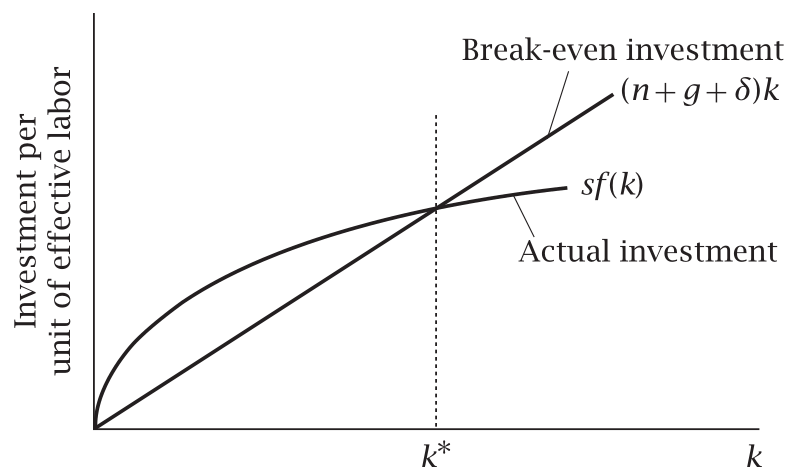
\includegraphics[width=0.6\textwidth]{image/s1.png}
    \caption{实际投资曲线与持平投资曲线}     \label{solows1}
\end{figure}

此外由定义消费等于产出减储蓄,$c_t = (1-s)y_t$,由于稳态下有效人均资本量$k^*$保持不变,故由生产函数的紧缩形式$f(k)$知此时有效人均产量$y^*$恒定为某一常数,故消费量$c^*$也将保持不变。

\begin{example}[$k^*$的黄金律值] \label{solowkgr}
    \mbox{} \\
    稳态下 
    \begin{equation*}
        sf(k^*) = (n+g+\delta)k^*.
    \end{equation*}
    有效人均消费量为
    \begin{align*}
        c^* & = (1-s)y^* \\
            & = f(k^*) - sf(k^*) \\
            & = f(k^*) - (n+g+\delta)k^*.
    \end{align*}
    对$c^*$关于$k^*$求一阶导
    \begin{align*}
        \frac{\partial c^*}{\partial k^*} & = f^\prime(k^*) - (n+g+\delta) .
    \end{align*}
    为使$c^*$最大,令上式为零,有
    \begin{align*}
        f^\prime(k^*) = (n+g+\delta)
    \end{align*}
    再根据$f(k)$的具体函数形式,我们就可得到$k_t$的黄金律值$k^*$。
    \footnote{假定生产函数为柯布-道格拉斯形式,即$y_t = k^\alpha$,则达到黄金律资本存量所需的储蓄率同为$\alpha$。参见课后习题1.5。}
\end{example}

\subsection{比较静态分析}

比较静态分析,即判断以及量化模型中外生参数变动对均衡状态下$k^*$和$c^*$的影响。
下面我们以储蓄率$s$的变动为例分析此类问题。

\subsubsection*{储蓄率$s$发生变动}
    \begin{enumerate}
        \item 对$k^*$的影响

                我们对均衡等式$s f\left(k^{*}(s, n, g, \delta)\right)=(n+g+\delta) k^{*}(s, n, g, \delta)$两端同时关于$s$求一阶导,
                    \begin{align}
                        s f^{\prime}\left(k^{*}\right) \frac{\partial k^{*}}{\partial s}+f\left(k^{*}\right) = 
                            (n+g+\delta) \frac{\partial k^{*}}{\partial s}
                    \end{align}
                整理得到
                    \begin{align}\label{solowpartialks}
                        \frac{\partial k^{*}}{\partial s} = \frac{f\left(k^{*}\right)}{(n+g+\delta)-s f^{\prime}\left(k^{*}\right)}
                    \end{align} 

        \item 对$y^*$的影响

                由$y=f(k)$,有
                    \begin{align}
                        \frac{\partial y^{*}}{\partial s} = 
                            f^{\prime}\left(k^{*}\right) \frac{\partial k^{*}(s, n, g, \delta)}{\partial s}
                    \end{align}
                将式(\ref{solowpartialks})结果带入,整理得到
                    \begin{align}
                        \frac{\partial y^{*}}{\partial s} = 
                            \frac{f^{\prime}\left(k^{*}\right) f\left(k^{*}\right)}{(n+g+\delta)-s f^{\prime}\left(k^{*}\right)}
                    \end{align}

        \item 对$c^*$的影响

                由定义,$c=(1-s)y$,且稳态下有$sf(k^*) = (n+g+\delta)k^*$,故得到
                    \begin{align}
                        c^{*} = f\left(k^{*}\right)-(n+g+\delta) k^{*}
                    \end{align}
                对其两端求导,整理得到
                    \begin{align}
                        \frac{\partial c^{*}}{\partial s} = 
                            \left[f^{\prime}\left(k^{*}(s, n, g, \delta)\right)-(n+g+\delta)\right] 
                            \frac{\partial k^{*}(s, n, g, \delta)}{\partial s}
                    \end{align}
                将式(\ref{solowpartialks})结果带入,得到
                \begin{align}
                        \frac{\partial c^{*}}{\partial s} = 
                            \left[f^{\prime}\left(k^{*}(s, n, g, \delta)\right)-(n+g+\delta)\right] 
                            \frac{f\left(k^{*}\right)}{(n+g+\delta)-s f^{\prime}\left(k^{*}\right)}
                    \end{align}
    \end{enumerate}

    同样,考察人口增长率$n$的变动对Solow稳态的影响也是依此步骤。
    由此我们可以总结道,求解比较静态分析问题时,
    第一步是找到该模型中有效人均资本存量的均衡等式,
    \footnote{在Solow模型中为$sf(k^*) = (n+g+\delta)k^*$),RCK中为资本动态方程与消费动态方程,OLG模型中直接为稳态下的有效人均资本解析式。
        需要特别注意的是,这三个模型关于资本折旧的假定存在差别,因此需要灵活调整资本动态方程中的持平投资项。}
    然后对其关于变动的外生参数求偏导,
    再根据生产函数性质及模型假定判断等式两边正负情况,即可得到$\partial k^* / \partial x$的正负,
    进而再对$y^* = f(k^*)$,$c^* = f(k^*) - (n+g)k^*$关于变动的外生参数求一阶导,
    藉由$\partial k^* / \partial x$的正负情况得到$\partial y^*/\partial x$和$\partial c^*/\partial x$的变动情况。
    即问题核心在于外生参数的变动对稳态下的有效人均资本$k^*$作何影响。



\section{Ramsey–Cass–Koopmans 模型}


与Solow模型中储蓄率$s$外生给定不同,在RCK模型中我们通过假设家庭效用函数,使得每一时刻家庭储蓄率$s_t$转化为内生变量。
背后的经济逻辑是,
\begin{itemize}
    \item 竞争性的厂商租赁资本、雇佣劳动力来进行生产并售出商品,同时按照生产要素的边际产出支付报酬;
    \item 家庭提供劳动并且持有资本,获得工资以及资本收益,决策消费和储蓄的分配比例。
\end{itemize}

\subsection{假设}

\begin{definition}[生产函数]
    关于生产函数的假设与Solow模型中的完全相同,
    \begin{equation}
        Y_t = F(K_t, A_t L_t)
    \end{equation}
    需要指出的是,由于我们分析的经济单位具体到了企业与家庭,
    故在RCK模型中我们需要考虑市场利率$r_t$与实际工资$w_t$。
\end{definition}

\begin{definition}[家庭效用函数]
家庭具有永久生命周期,且数量固定不变,面临的效用函数及预算约束为
    \begin{align}
        & \max U \,  = \int_{t=0}^{\infty} e^{-\rho t} \frac{C_t^{1-\theta}}{1-\theta} \frac{L_t}{H} dt \\
        & \, \mathrm{s.t.} \; \frac{K(0)}{H}+\int_{t=0}^{\infty} e^{-r_t}[W_t-C_t] \frac{L_t}{H} d t \geq 0
    \end{align}
    其中效用函数采取相对风险规避系数不变(CRRA)偏好,这是保证经济能够向平衡增长路径收敛的必要条件。
    \footnote{此时任意两个时间点间的消费替代弹性为$1/\theta$。参见课后习题2.2。}
    此外,为保证家庭终生效用不会发散,即禁止庞氏博弈,要求$\rho - n -(1-\theta)g > 0$.
\end{definition}

\begin{definition}[投入要素]
\begin{align}
    \mbox{人口增长率} \, \frac{\dot{L_t}}{L_t} = n, \quad
    \mbox{技术进步率} \, \frac{\dot{A}_t}{A_t} = g, \quad
    \mbox{折旧率} \, \delta = 0.
\end{align}
\end{definition}


\subsection{市场均衡}

\subsubsection*{厂商}

在完全竞争性市场中,厂商按生产要素的边际产出偿付报酬。
由于假定不存在折旧,资本的实际收益率就等于其单位时间收入,即资本的边际产出。
根据生产函数规模报酬不变假定,
我们可直接采用紧凑形式$f(k)$表达$t$时刻的市场利率,
\footnote{若存在资本折旧,则需从$r_t$中减去扣除资本折旧率$\delta$以得到市场实际利率。}
\begin{align}\label{ramseyr}
    \begin{aligned}
        r_t & = \frac{\partial F(K_t,A_t L_t)}{\partial \, K_t} \\
            & = \frac{\partial f(k_t)}{\partial \, k_t} \\
            & = f^\prime(k_t) .     
    \end{aligned}
\end{align}
单位劳动的平均工资为
\begin{align}
    \begin{aligned}
        W & = \frac{\partial F(K,AL)} {\partial L} \\
        & = A \frac{\partial F(K,AL)} {\partial AL} \\
        & = A \left[f(k) - k \frac{\partial F(K,AL)} {\partial K} \right] \\
        & = A \left[f(k) - k f^\prime(k) \right] .
    \end{aligned}
\end{align}
故$t$时刻每单位有效劳动实际工资$w_t = f(k_t) - k_t f^\prime(k_t)$.
\footnote{$f\left(x_{1} x_{2} \ldots x_{n}\right)$ 为 $r$次齐次方程,则有
        \begin{align*}
            \frac{\partial f}{\partial x_{1}} x_{1} + 
            \frac{\partial f}{\partial x_{2}} x_{2} \ldots + 
            \frac{\partial f}{\partial x_{n}} x_{n} 
                \equiv r f\left(x_{1}, x_{2}, \ldots x_{n}\right),
        \end{align*}
            我们在前面假定生产函数规模报酬不变,即此处$r=1$.
            }

\subsubsection*{家庭}

由家庭效用最大化,得有效人均消费的动态方程。
        \begin{align}
          \begin{aligned}
            & \max_{c_t} U = B\int_{t=0}^\infty e^{-\beta t} \frac{c_t^{1-\theta} }{1-\theta} dt, 
            \quad B=\frac{A_0^{1-\theta} L_0}{H},
            \quad \beta = \rho - (1-\theta)g - n. \\ 
            & \, \mathrm{s.t.} \quad k_0 + \int_{t=0}^\infty e^{-R_t + (n+g)t} (w_t - c_t) dt = 0,
            \quad R_t = \int_{s=0}^t r_s ds.
          \end{aligned}
        \end{align}
        构造Lagrange函数
        \footnotetext{也可采用现值Hamiltonian函数法。}
        \begin{equation}
            \mathcal{L} = B\int_{t=0}^\infty e^{-\beta t} \frac{c_t^{1-\theta} -1}{1-\theta} dt +
                \lambda \left[k_0 + \int_{t=0}^\infty e^{-R_t + (n+g)t} (w_t - c_t) dt\right]
        \end{equation}
        F.O.C
        \begin{equation}
              \frac{\partial \mathcal{L}}{\partial c_t} = 
                     B e^{-\beta t} \mathcal{C}_t^{-\theta} - \lambda e^{-R_t} e^{(n+g) t} = 0
        \end{equation}
        对其两端取对数
        \begin{align}
            \begin{aligned} 
                \ln B-\beta t-\theta \ln c_t &= \ln \lambda-R_t+(n+g) t \\ 
                    &= \ln \lambda-\int_{\tau=0}^{t} r(\tau) d \tau+(n+g) t 
            \end{aligned}
        \end{align}
        再同时关于时刻$t$求导数
        \begin{align}
            -\beta-\theta \frac{\dot{C}_t}{C_t}=-r_t+(n+g)
        \end{align}
        化简有
        \begin{align} 
            \begin{aligned} 
                \frac{\dot{c}_t}{c_t} &=\frac{r_t-n-g-\beta}{\theta}                          
            \end{aligned}
        \end{align}
        带入$\beta = \rho - (1-\theta)g - n$,
        \begin{align} \label{ramseygc}
            g_c^* \equiv \frac{\dot{c}_t}{c_t}= \frac{r_t-\rho-\theta g}{\theta}
        \end{align}
        
        由式中结果,我们得知有效人均消费增长率取决于市场实际利率$r_t$,与人口增长率$n$无关。
        带入上述式(\ref{ramseyr})结果,令$r_t=f^\prime(k_t)$,则有效人均消费增长率为
            \begin{equation}
                g_c^*  = \frac{f^\prime(k_t) - \rho}{\theta} - g
            \end{equation}

\subsection{均衡配置} 

    由假定$f^{\prime \prime}(k) < 0$,资本边际生产率呈现递减规律,故在RCK模型中,
    随着有效人均资本的累积,有效人均消费量增长率$g_c^*$最终将稳定在\textcolor{red}{零值}。
    同时根据定义,当期资本变化量为该期产出$f(k_t)$减去消费$c_t$以及持平投资$(n+g)k_t$。
    因此RCK模型中的资本动态方程为
    \begin{align}  \label{ramseygky}
        \dot{k}_t & = f(k_t) - c_t - (n+g)k_t \\ 
                & = r_tk_t + w_t - c_t - (n+g)k_t 
    \end{align}

    \begin{proof}{BGP上有效人均消费增长率等于有效人均资本增长率}
    \mbox{} \\
    对上式两端同除以$k_t$,得到
    \begin{align}
        g_{k_t} \equiv \frac{\dot{k}_t}{k_t} = r_t + \frac{w_t}{k_t} - \frac{c_t}{k_t} - (n+g)     \label{ramseygkk}
    \end{align}
    由上述消费动态方程我们知道,RCK模型中BGP上$k_t$固定为$k^*$,
    故有效劳动平均工资$w_t$同样固定为$w^* = f(k^*) - k^* f^\prime(k^*)$,
    此时要令等式(\ref{ramseygkk})中左端为常数,则右端$c_t/k_t$也必要为某一个常数。
    故在BGP上,
    \begin{align}
        c_t = \gamma \, k_t, \quad \gamma \ \mbox{为某一常数}
    \end{align}
    对上式两端同时取自然对数,并关于时间$t$求导,我们得到
    \begin{align}
        \frac{\dot{c}_t}{c_t} = \frac{\dot{k}_t}{k_t}
    \end{align}
    由于在BGP上$g_{c}^*=0$,故
    \begin{align}
        g^*_k = g^*_c =0
    \end{align}
    此即RCK的市场竞争均衡与BGP。
    \end{proof}

    由于在BGP上有效人均资本存量$k_t$恒定为由消费动态方程$g_{c_t}^*=0$决定的$k^*$。
    若再给定生产函数具体形式以及参数$g$、$\rho$、$\theta$,
    我们就可由式$f^\prime(k^*) = \rho + \theta g$
    直接求得该BGP上的有效人均资本存量$k^*$的解析式(或具体值)。
    相继地,如图~\ref{ramseyequipoint}所示,透过$\dot{k}_t = 0$曲线$k^*$进一步决定了$c^*$的取值。
    代数上,由式 $c^*=f(k^*)-(n+g)k^*$ 可直接得到有效人均消费量 $c^*$。
    反映在图像上即为图~\ref{ramseyequipoint}中的均衡点E。

    综上所述,给定初始有效人均资本量$k_0$和初始有效人均消费量$c_0$,经过一段时间调整,
    单位有效劳动的平均资本、平均产出和平均消费的增长率都为常数0,
    该经济体通过市场机制到达BGP。
    并且同Solow模型一样,
    储蓄率$ s= (y^* - c^*)/ y^*$为固定常数。

\begin{note}[计算逻辑]
    由于这里涉及的知识点与计算量不少,因此极易出考题,
    有必要再强调一下变量均衡值的计算逻辑:
    \textcolor{red}{
    由生产函数得市场实际利率,
    由消费动态方程得$k^*$值,
    继而得到单位有效劳动平均产出$y^* = f(k^*)$,
    再由资本动态方程得$c^*$值。}
\end{note}

\begin{figure}[!htbp]
    \centering
    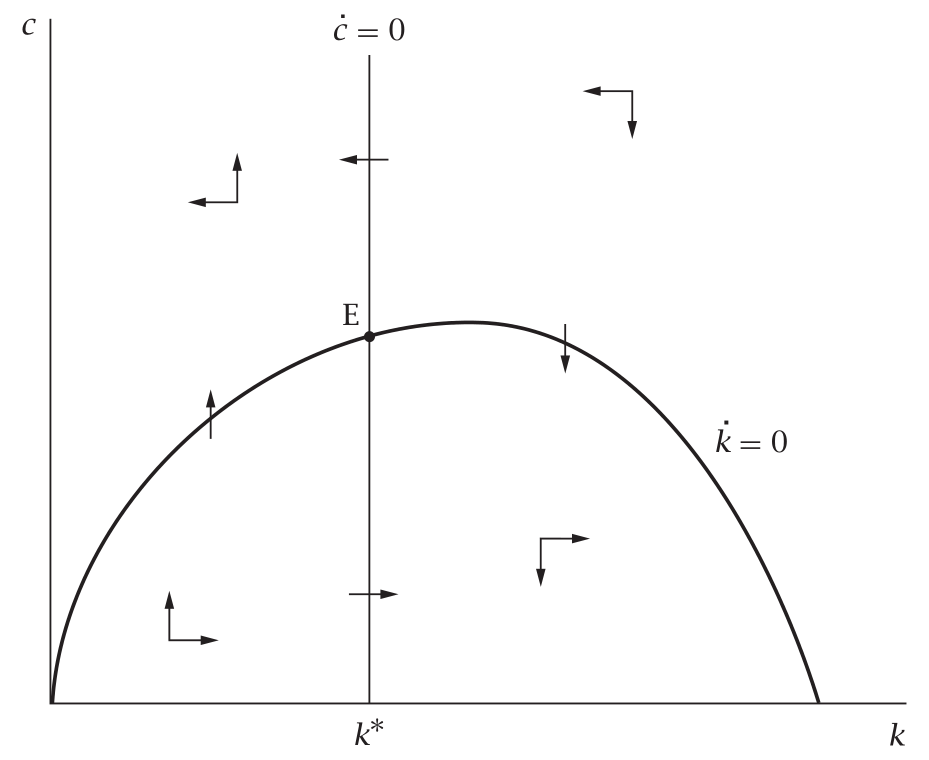
\includegraphics[width=0.5\textwidth]{image/r3.png}
    \caption{动态$c$与$k$}     \label{ramseyequipoint}
\end{figure}

\begin{proof}{图~\ref{ramseyequipoint}中的E点位于$\dot{k} = 0$曲线顶点的左端}
        \footnote{图中$\dot{k} =0$曲线上每一点皆代表可能的BGP路径。
        并且从AK开始,由于持续的技术进步,有效人均消费量增长率为大于零的固定常数,再计算$c_t$则需使用积分方法。}

    由消费动态方程$g_{c_t}^* =0$,我们得到$k^*$的值
    \begin{align*}
        f^\prime(k^*) = \rho + \theta g
    \end{align*}
    而由定义稳态下有效人均消费量等于产出减去持平投资,即
    \begin{align*}
        c_t = f(k_t) - (n+g)k_t
    \end{align*}
    对等式两边关于$k$求导
    \begin{align*}
        \frac{\partial c_t}{\partial k_t} = f^\prime(k_t) - n - g
    \end{align*}
    为使消费最大,令其一阶导数等于零
    \begin{align*}
        \frac{\partial c_t}{\partial k_t} = 0
    \end{align*}
    我们得到$k^{GR}$
    \begin{align*}
        f^\prime(k^{GR}) = n+g
    \end{align*}
    之前为保证家庭终生效用不会发散,有假定
    \begin{align*}
        \rho - n - (1-\theta)g >0
    \end{align*}
    移动不等式左右两端项,有
    \begin{align*}
        f^\prime(k^*) = (\rho + \theta g) > (n+g) = f^\prime(k^{GR})
    \end{align*}
    由于生产函数中已有定义$f^{\prime \prime}(k) < 0$,故有
    \begin{align*}
        k^* < k^{GR}
    \end{align*}
    得证BGP上$k^*$小于使得有效人均消费$c$最大的$k^{GR}$。
\end{proof}

\subsection{相图中的动态学}
 
下面我们根据图~\ref{ramseyequipoint}、图~\ref{ramseyr4}以及图~\ref{ramseyr5}
来分析效用折现率$\rho$的减小对BGP上$k^*$与$c^*$的影响。
\footnote{若政府对工资收税,消费动态方程与资本动态方程作何变动?2018年期末试卷真题。}
当外生参数$\rho$减小时(因为效用折现率决定了消费者对于跨期消费的意愿强度,故类似于Solow模型中的储蓄率上升),
由消费动态方程表达式
\begin{align*}
    g_{c_t} = \frac{r_t - \rho}{\theta} - g
\end{align*}
我们知,此时要令经济收敛于BGP,即$r_t - \rho - \theta g = 0$,则$r_t$值必然要随之同方向等程度变动。
而$r_t = f^\prime(k_t)$,$f^{\prime \prime}(k_t) <0$。则新BGP上的$k^*_{new}$ 必然要大于之前的$k^*_{old}$,
故当下经济中的个体将选择减少消费,增加储蓄,以提高有效人均资本量。
于是图~\ref{ramseyequipoint}中的$\dot{c}$线将向右移动。

资本动态方程
\begin{align*}
    \dot{k}_t = f(k_t) - c_t - (n+g)k_t
\end{align*}
则告诉我们,要令$\dot{k}_t > 0$,有效人均消费量必然要减少,故有效人均消费量$c_t$将跳跃性减小,
反应在图~\ref{ramseyr4}中则为$c_t$从B点立即下降到F点。
此后,由于$\dot{k}_t > 0$,$k_t$值将从图中的$k(0)$缓慢并且连续地移动到$k^*$处。
相应的有效人均消费量$c_t$也由于$k_t$的增大而逐渐提高。
因此,逻辑上是消费最开始的跳跃性调整以及随后的连续性调整使得资本存量得到连续性调整。
最后,经济平稳过渡到新的BGP,即图中的E点。
\footnote{参见Romer版教材课后习题2.10、2.11。}

需要注意的是,
如图~\ref{ramseyequipoint}所示,不同初始$c_0$值下仅有F点能收敛于新的BGP。
即对于任意一个大于零的初始$k_0$值,仅存在唯一一个$c_0$值使得家庭跨期最优化条件、
资本存量动态学、家庭预算约束以及$k_t$不能为负的条件同时得到满足。
若我们将初始$k_0$与$c_0$值一一建立联系,则得到图~\ref{ramseyr5}中的鞍点路径。
显然,每当经济遭遇外来冲击时,为求BGP,调整的下一期有效人均消费量$c$必要落于图~\ref{ramseyr5}中的鞍点路径上。

\begin{figure}[!htbp]
    \centering
        \begin{minipage}[t]{0.48\textwidth}
            \centering
            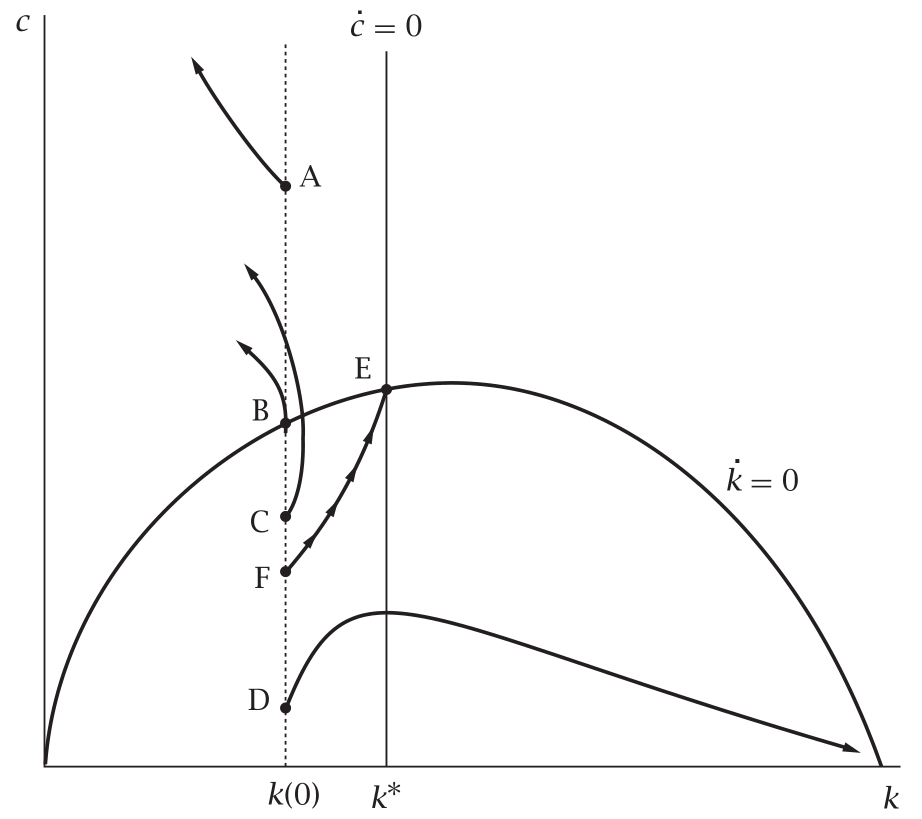
\includegraphics[width=6cm]{image/r4.png}
            \caption{不同初始$c_0$下的$c_t$、$k_t$}  \label{ramseyr4}
        \end{minipage}
        \begin{minipage}[t]{0.48\textwidth}
            \centering
            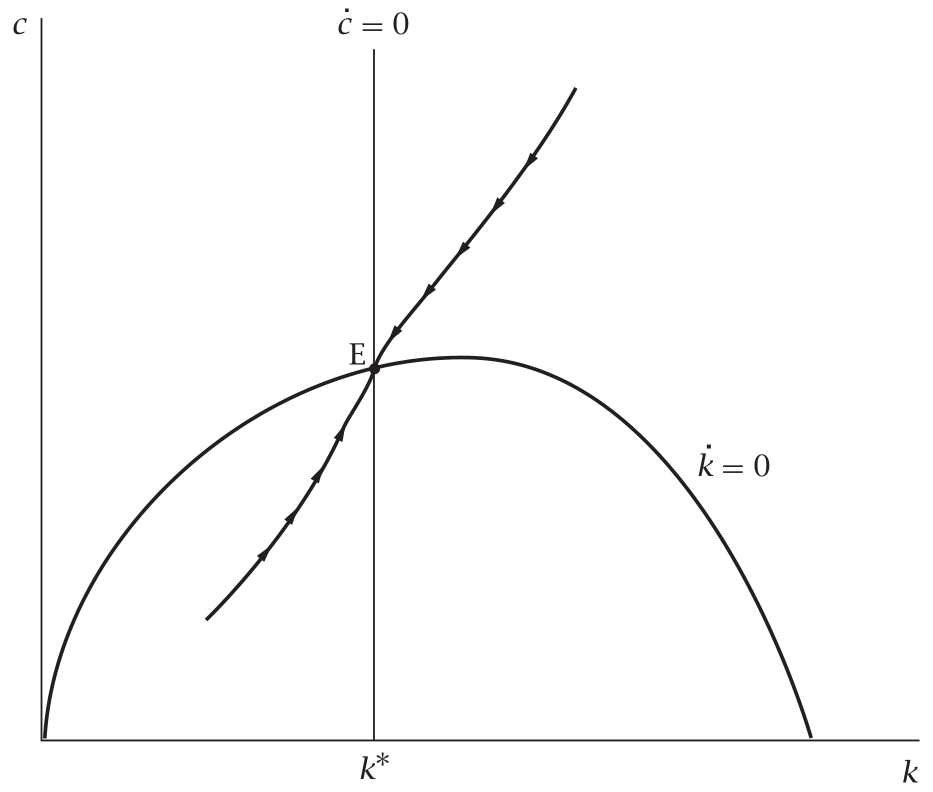
\includegraphics[width=6cm]{image/r5.png}
            \caption{鞍点路径}     \label{ramseyr5}
        \end{minipage}
\end{figure}

\begin{remark}
    完全竞争性市场下,企业按生产要素的边际产出偿付报酬,加上规模报酬不变假设,则企业利润为零,
    资本所得与劳动收入相加就等于产出,$r_t k_t + w_t \equiv y_t$。
    而资本$k$和劳动皆由家庭持有,
    故此时经济中消费和储蓄的分配比例完全取决家庭决策(政府没有做出政策调整时)。
    我们知道家庭消费决策建立在效用最大化基础之上,
    而通过消费动态方程(\ref{ramseygc})式我们可以看出
    各期有效人均消费量$c_t$实际取决于消费者面对市场实际利率$r_t$和自身的跨期消费偏好$\rho$的权衡比较,
    即家庭通过跨期配置当前与未来的消费达到效用最大化。
    调节的基础是市场利率$r_t$、效用折现率$\rho$,以及预算约束$f(k_t) \geq c_t + (n+g)k_t$。
    最终,经济体在$g_{c_t}^*$为某一常数(大于等于零)时达到BGP。
\end{remark}

      
\section{Diamond overlapping-generations 模型}
    
在RCK模型的基础上,戴蒙德世代交叠模型考虑人口的新老更替,即经济中青年个体不断出生,老的个体不断衰亡。
因此,此模型核心在于是将新老交替假设体现在效用函数和资本动态方程中。

\subsection{假设}

\begin{definition}[生产函数]
    关于生产函数的假设与前面RCK模型完全相同。
    \begin{equation}
        Y_t = F(K_t, A_t L_t).
    \end{equation}
\end{definition}

\begin{definition}[个人效用函数]
    仍假设效用函数的风险规避系数是常数。
    由于寿命有限假设的存在,我们不再需要假定$\rho - n - (1-\theta)g > 0$来确保个人终生效用不发散。
    
    令$C_{1,t}$和$C_{2,t}$分别表示第$t$期年轻人和老年人的消费,
    出生于$t$期的人面临预算约束——两期消费的现值之和等于终生劳动收入,
    于是他们的效用函数和预算约束式可表示为
    \footnote{若将利率替换为价格,预算约束式又该怎么写? 参见课后习题2.2。2018年期末试卷原题。}
    \begin{align}
        & \max \, U = \frac{C_{1,t}^{1-\theta}}{1-\theta} + \frac{1}{1+\rho} \frac{C_{2, t+1}^{1-\theta}}{1-\theta}  \\ 
        & \, \mathrm{s.t.} \;  C_{1,t} + \frac{1}{1+r_{t+1}} C_{2,t+1} \le A_t w_t
    \end{align}   
    经济个体目标是最大化两期效用之和,这受制于其老年期的市场利率$r_{t+1}$和其主观效用折现率$\rho$。
\end{definition}

\begin{definition}[投入要素]
\begin{align}
    \mbox{人口增长率} \, \frac{\dot{L_t}}{L_t} = n, \quad
    \mbox{技术进步率} \, \frac{\dot{A}_t}{A_t} = g, \quad
    \mbox{折旧率} \, \delta = 0.
\end{align}
\end{definition}

\subsection{市场均衡}

跟据个体效用最大化原则,建立Lagrange方程
\begin{align}
    \mathcal{L}( C_{1,t}, C_{2,t+1}, \lambda) =
        \frac{C_{1,t}^{1-\theta}}{1-\theta}+\frac{1}{1+\rho} \frac{C_{2, t+1}^{1-\theta}}{1-\theta} + 
        \lambda\left[A_{t} w_{t}-\left(C_{1,t}+\frac{1}{1+r_{t+1}} C_{2,t+1}\right)\right]
\end{align}
F.O.C
\begin{align}
    \mathcal{L}_{C_{1,t}} & = 0 \\
    \mathcal{L}_{ C_{2,t+1}} & = 0
\end{align}
即有
\begin{align}
    C_{1 t}^{-\theta} & = \lambda \\ 
    \frac{1}{1+\rho} C_{2 t+1}^{-\theta} & = \frac{1}{1+r_{t+1}} \lambda
\end{align}
得到两期消费量之比
\begin{equation}
    \frac{C_{2,t+1}}{C_{1,t}} = \left( \frac{1+r_{t+1}}{1+\rho}\right)^{1/\theta}
\end{equation}
将之带入预算约束式,得到
\begin{align}
    C^*_{1,t} & = \frac{(1+\rho)^{1/\theta}}{(1+\rho)^{1/\theta} + (1+r_{t+1})^{(1-\theta)/\theta}} A_t w_t \\
    C^*_{2,t+1} & = \frac{(1+ r_{t+1})^{1/\theta}}{(1+\rho)^{1/\theta} + (1+r_{t+1})^{(1-\theta)/\theta}} A_t w_t 
\end{align}
故有内生储蓄率
\footnote{需要指出的是,个人年轻期储蓄量的多少取决于老年期的利率,即其权衡个人效用折现率与市场实际利率从而实现个人效用最大化。
          在实际BGP计算中,有$k_t = k^*$, $r_t = f^\prime(k^*)$,前后期利率相等,故实质上并不影响计算结果。}
\begin{align}\label{olgk}
\begin{aligned}
    s(r_{t+1}) & = 1 - \frac{C_{1,t}}{A_t w_t} \\
           & = \frac{(1+r_{t+1})^{(1-\theta)/\theta}}{(1+\rho)^{1/\theta} + (1+r_{t+1})^{(1-\theta)/\theta}}    
\end{aligned}
\end{align}

\subsubsection*{资本动态方程}

出生于$t$期的青年人参与劳动,工资$A_t w_t$被分配于当期消费与储蓄。
与此同时,$t$期的老年人(即$t-1$期的年轻人)不再参与劳动,只凭借储蓄与资本利得生活,
并于$t$期末消耗完所有财产退出经济。
于是,$t+1$期的资本存量$K_{t+1}$就等于$t$期的年轻人数量$L_t$乘以其储蓄量$A_t w_t - C_{1,t}$。
若采用储蓄率的形式,则表现为
    \begin{equation}
        K_{t+1} = s(r_{t+1}) L_t A_t w_t
    \end{equation}
对上式两端同时除以$A_{t+1} L_{t+1}$,得到有效劳动人均资本
\begin{align}
    \begin{aligned} \label{olgmk}
        k_{t+1} & = \frac{1}{(1+n)(1+g)} s(r_{t+1}) w_t \\
                & = \frac{1}{(1+n)(1+g)} s(f^\prime(k_{t+1})) \left[f(k_t) - k_t f^\prime(k_{t})\right]
    \end{aligned}
\end{align}
令$k_{t+1} = k_t$,再带入市场实际利率和有效劳动收入,就可得到$k^*$的解析式。
\footnote{OLG模型的比较静态分析即是再对$k^*$的解析式求偏导。}

\subsection{动态无效率}

对各世代人口的效用函数做线性变化,
\begin{align}
    U = \frac{C_{1,t}^{1-\theta} -1}{1-\theta} + \frac{1}{1+\rho} \frac{C_{2, t+1}^{1-\theta} -1}{1-\theta}
\end{align}
由于只是加减了常数,与原效用函数式相比并无实质性改变。令$\theta =1$,
我们发现其极限为$0/0$型函数,应用洛必达法则,对分子分母同时关于$\theta$求导,
\begin{align}
U = \frac{- \, C_{1,t}^{1-\theta} \, \ln C_{1,t}}{-1} + \frac{1}{1+\rho} \frac{- \, C_{2, t+1}^{1-\theta} \ln C_{2,t+1}}{-1}
\end{align}
带入$\theta =1$,有
\begin{align}
U =  \ln C_{1,t} + \frac{1}{1+\rho} \ln C_{2,t+1}
\end{align}
即效用函数转变为对数形式。
为使运算方便,令外生技术进步率$g=0$,生产函数具体形式为Cobb-Douglas生产函数$f(k)=k^\alpha$,
带入式(\ref{olgmk})得到
\begin{align}
k^{*}=\left[\frac{1}{1+n} \frac{1}{2+\rho}(1-\alpha)\right]^{1 /(1-\alpha)}
\end{align}

再回过头来计算使得消费最大(福利水平最高)的有效人均资本存量。
在BGP上,由资本动态方程$\dot{k}_t =0$可知,
单位有效劳动的平均消费为
\begin{align}
c^* = f(k^*) - (n+g) k^*
\end{align}
若使有效人均资本存量$k^*$保持在黄金律水平,由于已假设$g=0$,则需$f^\prime(k^{GR}) = n$,即
\begin{align}
k^{GR} = \left(\frac{\alpha}{n}\right)^{1/(1-\alpha)}
\end{align}

我们发现随着$\alpha$取不同值,$k^*$既可能大于$k^{GR}$,也可能小于$k^{GR}$。
特别地,当$\alpha$充分小时,平衡增长路径上的有效人均资本存量大于黄金律水平,$k^* > k^{GR}$。
此时我们判定OLG模型中的BGP非Pareto有效状态,政府可以推行政策促使$k^*$减小并保持在$k^{GR}$水平。

\begin{figure}[!htbp]
    \centering
    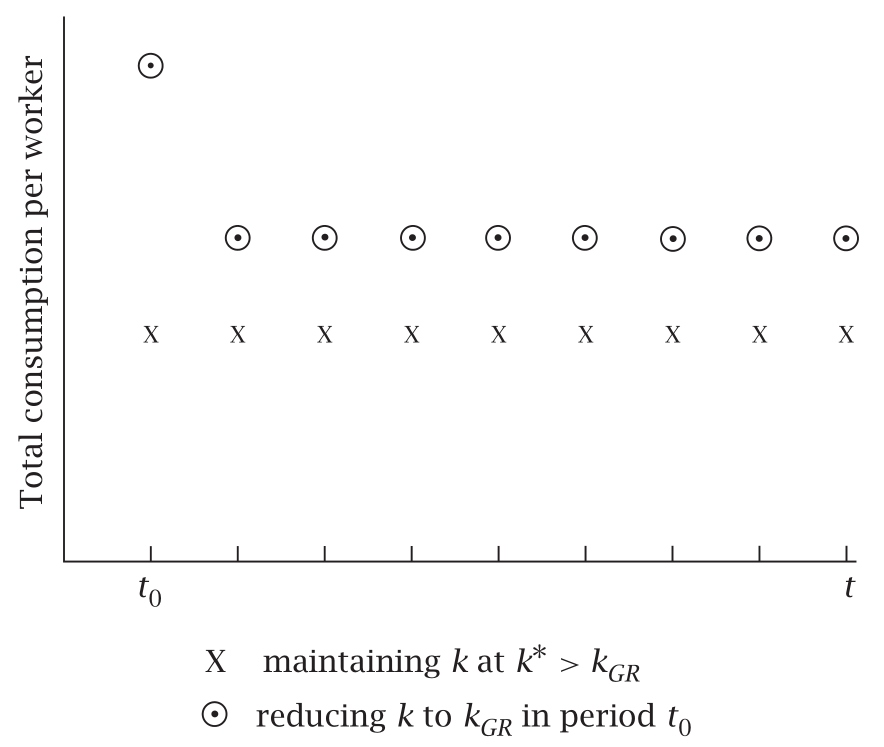
\includegraphics[width=0.5\textwidth]{image/olg1.png}
    \caption{有效劳动平均消费路径的转变($k^*$降低到黄金律水平$k^{GR}$)}     \label{olg1}
\end{figure}

如上图所示,$X$表示有效人均资本维持在$k^*$时的有效人均消费$c^*$,$\odot$表示有效人均资本维持在黄金律水平$k^{GR}$时的最大消费。
假设在$t_0$时刻,政府出台一项政策,如降低存款储蓄率,促使消费者将其收入更多地分配给当前期消费,从而使得$t_0$期往后有效人均资本量降为$k^{GR}$。
用代数形式表示,则$t_0$期,有效劳工的消费水平为
\begin{align}
c^p_{t_0} = f(k^*) - nk^{GR} + (k^* - k^{GR})
\end{align}
而在接下来每一时期(BGP),有效人均消费量为
\begin{align}
c^p_{t} = f(k^{GR}) - n k^{GR}
\end{align}
由于$k^{GR}$能使$f(k) -nk$最大化,故
\begin{align}
f(k^{GR}) - nk^{GR} > f(k^{*}) - nk^{*}
\end{align}
即$\odot$位于$X$之上。
同时由于$k^* > k^{GR}$,有
\begin{align}
\left[ f(k^{*}) - nk^{GR} + (k^* - k^{GR}) \right]> f(k^{GR}) - nk^{GR}
\end{align}
即$t_0$时刻的有效人均消费量比黄金律水平还要高。
表示在上图中即为$t_0$时刻的$\odot$“会当凌绝顶,一览众山小。”

\subsection{社会计划者}  \label{socialplanolg}

社会计划者面临的优化问题为最大化当期所有世代人口的消费
\footnote{2019年期末试卷真题。}
\begin{align}
    \max_{\{C_1,C_2\}} U(C_1,C_2) = C_1 + \frac{1}{1+n} C_2
\end{align}

其面临的约束为当期消费与储蓄量不能超出当期产出,
\begin{align}
    Y_t \le (L_t A_t c_1 + L_{t-1} A_t c_2) +  (L_{t+1} A_t k_{t+1} - L_t A_t k_t)
\end{align}
等式右端第一个括号内为当期消费,第二个括号内为当期储蓄(对社会计划者而言,不存在价格调整与利率问题)。

假设生产函数为Cobb-Douglas生产函数,$f(k)=k^\alpha$.
此外为方便运算,令外生技术进步率$g=0$,$\theta = 1$。
根据式(\ref{olgk}),此时个人储蓄率$s = 1/(2+\rho)$,不依赖于市场利率,只与效用折现率$\rho$有关。
其余条件与前述假定相同。

对总预算约束除以有效劳动人口数$A L_t$,得有效人均资本约束条件
\begin{align}
    k_t^\alpha = c_1 + \frac{1}{1+n}c_2 + (1+n)k_{t+1} - k_t
\end{align}
当达到均衡状态时有$\dot{k}_t = 0$,即$k_{t+1} = k_t$,
将此条件带入资本约束方程得
\begin{align}
    (k^s)^\alpha = c_1 + \frac{1}{1+n} c_2 + n k^s
\end{align}
两端关于$k^s$求偏导,等式仍然成立
\begin{equation}
  \alpha (k^s)^{\alpha -1} = n
\end{equation}
化简有
\footnote{
求解下列最优化问题可得到相同结果,
\begin{align*}
    & \max \, U  = C_{1,t} + \frac{1}{1+n} C_{2,t} \\
    & \, \mathrm{s.t.} \; k_t^\alpha - c_1 - \frac{1}{1+n}c_2 - (1+n)k_{t+1} + k_t \geq 0
\end{align*}}
\begin{equation}
    k^s = \left(\frac{\alpha}{n} \right)^{1/(1-\alpha)}
\end{equation}
即我们由稳态下$\dot{k}_t = 0$这一条件直接得到$k^s$的表达式。

易证,当$0< \alpha < \frac{n}{n + (1+n)(2+\rho)} <1$时,
前述假定下市场决定的有效人均资本量$k^*$大于社会计划者下的$k^{s}$
\begin{align}
    k^* = \left(\frac{ 1- \alpha}{(1+n)(2+\rho)} \right)^{1/(1-\alpha)} > 
        \left(\frac{\alpha}{n} \right)^{1/(1-\alpha)}
\end{align}
由于此时储蓄率$s$固定为$1/(2+\rho)$,较大的人均资本存量拥有较大的人均产出与较大的人均消费量,
故社会计划者指挥下的BGP存在效率改进空间。

\quad \newline

以上内容出自 David Romer 的 Advanced Macroeconomics (4th edition) 第一、二两章。
下面列出原始文献,既是强调出处,另可供学有余力者阅读。

\subsection*{The Solow Model}

\href{http://www.jstor.org/stable/1884513}
{Robert M. Solow, A Contribution to the Theory of Economic Growth. 
Quarterly Journal of Economics 70 (February 1956), 65–94.}

\href{http://www.jstor.org/stable/2006549}
{Robert E. Lucas, Jr., “Why Doesn’t Capital Flow from Rich to Poor Countries?”
American Economic Review 80 (May 1990), 92–96.}

\href{http://www.jstor.org/stable/1807174}
{J. Bradford DeLong, “Productivity Growth, Convergence, and Welfare: Comment,”
American Economic Review 78 (December 1988): 1138–1154.}

\subsection*{The Ramsey-Cass-Koopmans Model}

\href{http://www.econ.berkeley.edu/~obstfeld/ftp/perplexed/cts4a.pdf}
{Maurice Obstfeld, “Dynamic Optimization in Continuous-Time Economic Models
(A Guide for the Perplexed),” unpublished paper, U.C. Berkeley, April 1992.}

Robert J. Barro and Xavier Sala-i-Martin, Economic Growth, second edition
(Cambridge: MIT Press, 2004), Chapter 2 and Appendix A.3.

Lars Ljungqvist and Thomas J. Sargent, Recursive Macroeconomic Theory, second
edition (Cambridge: MIT Press, 2004), Chapter 3.

\newpage

\begin{remark}
    在前面我们学习了Solow模型、RCK模型以及OLG模型,得到的结论是在BGP上有效人均消费增长率恒为零。
    即受生产要素边际生产率下降约束,经济增长只来源于人口增长和外生技术进步率$g$。
    
    之后内生经济增长部分来源于 Acemoglu 的 \textit{Introduction to Modern Economic Growth} 第2、11、12、13、14章。
    我们先通过假设生产函数形式为$Y_t = A K_t$,其中$A$为大于零的常数,突破资本的边际生产率递减趋势,
    得到我们想要的$c_t^*$的长期永续增长。
    但由于该假设过于牵强,只是数学上的技巧,不符合经济规律,于是我们退一步假设:
    产品分为最终品和中间品两类,其中中间品作为一类资本用于最终品的生产。
    且为了易于理解并且方便计算,
    我们将中间品假设为参与生产的唯一资本要素,代替$K$的位置,并且是一次性消耗品。
    在此假定之下,我们得到预期结论——是技术进步,如中间品种类扩增和质量提升,使得经济具有永续增长效应。
    
    从模型设计来看,AK模型、种类扩张模型以及质量阶梯模型实质上都是为了在模型内部找到经济增长源泉,
    以走出生产要素边际报酬递减带来的Solow稳态。
    也就是说,假设中间品总种类为$N_t$,平均质量为$Q_t$,
    在相当长一段时期内若$N_t$或$Q_t$的增长率稳定在常数$\zeta$,
    则在通过市场机制或社会计划达到的BGP上,人均消费增长率$g_c^*$也始终为$\zeta$。
    不再依赖于之前外生给定的技术进步率$g$。
\end{remark}

\subsection*{Endogenous Growth Theory}


\href{http://www.jstor.org/stable/2937632}
{Paul M. Romer, “Endogenous Technical Change,” Journal of Political Economy 98
(October 1990, Part 2), S71–S102.}

\href{http://dx.doi.org/10.1016/0304-3932(88)90168-7}
{Robert E. Lucas, Jr., “On the Mechanics of Economic Development,” Journal of
Monetary Economics 22 (July 1988) 3–42.}


\section{AK-Ramsey}
    
\subsection{假设}

\begin{definition}[生产函数]
    假定总生产函数形式为
    \begin{equation}
        Y_t = A K_t, \quad A > 0.
    \end{equation}
    该生产函数不再包含劳动要素,
    故劳动收入$w$为零,可理解为要素市场中劳动力无弹性供给。
\end{definition}
\begin{definition}[个人效用函数]
    效用函数则延续RCK模型中的形式,
    \begin{align}
        & \max \, U  = \int_{t=0}^{\infty} e^{-(\rho - n)t} \frac{c_t^{1-\theta} -1}{1-\theta}  d \, t, \\
        & \, \mathrm{s.t.} \; \dot{a}_t =  y_t - c_t - (r_t - n)a_t + w_t
    \end{align}
    但有效人均资本$k_t$重新定义为人均财富$a_t$。
    并且与资本动态方程形成对比,个人财富动态方程中无折旧成分,在计算实际利率时不要遗漏扣除折旧率的步骤。
    需要注意,\textcolor{red}{从AK模型开始我们去掉外生假定的外生技术进步率$g$,不再有有效人均概念。
    小写字母$c$与$w$的重新定义为人均消费与人均收入。}
    \footnote{之所以有此重新定义,是因为Romer版教材中用大写字母表示人均量,用小写字母表示有效人均量,但Acemoglu版教材中直接使用小写字母表示人均量。}
\end{definition}
\begin{definition}[投入要素]
    \begin{align}
        \mbox{人口增长率} \, \frac{\dot{L_t}}{L_t} = n, \quad
        \mbox{折旧率} \, \delta > 0.
    \end{align}
\end{definition}

\subsection{市场均衡}

市场中资本的边际产出为
\begin{align}
\begin{aligned}
    \frac{\partial Y_t}{\partial K_t} = \frac{\partial AK_t}{\partial K_t} = A
\end{aligned}
\end{align}
由于存在折旧,故市场实际利率为
\begin{align}\label{AKRamr}
\begin{aligned}
    r_t = A - \delta  
\end{aligned}
\end{align}

求解个人效用最大化问题,构造现值Hamiltonian函数
\begin{equation}
    \hat{H}( c_t, a_t, \mu) = \frac{c_t^{1-\theta}-1}{1-\theta} + 
                         \mu\left[(r-n)a_t - c_t \right]
\end{equation}
F.O.C
\begin{align}
    \hat{H}_{c_t} & =0 \\ 
    \hat{H}_{a_t} & = -\dot{\mu} +  (\rho - n) \mu
\end{align}
分别可得
\begin{align}
    \frac{\dot{c}_t}{c_t} & = -\frac{1}{\theta} \frac{\dot{\mu}}{\mu} \\ 
    \frac{\dot{\mu}}{\mu} & = -r + \rho
\end{align}
从而得到有效人均消费增长率
\footnote{此即现值汉密尔顿函数的统一形式,往后直接套用就行。
        不过需要谨记,RCK模型中$g_c^*$需减去$g$.}
\begin{align}\label{AKRamgc}
    g^*_c \equiv \frac{\dot{c}_t}{c_t} = \frac{r_t - \rho}{\theta} 
\end{align}
综合(\ref{AKRamgc})式与(\ref{AKRamr})式,即将市场实际利率带入消费动态方程,我们得到
\begin{align}
    g^*_c =\frac{1}{\theta}(A-\delta-\rho)
\end{align}
此时由于$A,\delta,\rho$均为常数,故该均衡状态也为BGP。
若要保证该经济体有正的增长率,则需假定$A > \rho + \delta$. 
同时,由家庭消费收敛条件$\rho - n - (1-\theta)g >0$, 
知此时有隐性条件$\rho > (1-\theta)(A-\delta) + \theta n$.

\subsection{均衡配置}
均衡状态下,资本动态方程
\begin{equation}
    g^*_{k_t} \equiv \frac{\dot{k}_t}{k_t} = (A-\delta - n) - \frac{c_t}{k_t}
\end{equation}
    应为常数,故等式右边$c_t/k_t$需为常数,这要求
\begin{equation}
     g^*_k =g_c^* = \frac{A - \delta - \rho}{\theta}
\end{equation}
故有均衡配置
\begin{align}
    k_t & = k_0 \; \mbox{exp} \left( \frac{1}{\theta} (A-\delta - \rho) t \right), \\
    c_t & = c_0 \; \mbox{exp} \left( \frac{1}{\theta} (A-\delta - \rho) t \right).
\end{align}
再回到资本动态方程
\begin{align}
    \dot{k}_t=(A-\delta-n) k_t-c_0 \exp \left(\frac{1}{\theta}(A-\delta-\rho) t\right)
\end{align}
积分可得
\begin{align}
    \begin{aligned} 
        k_t & = \left[(A-\delta)(\theta-1) \theta^{-1}+\rho \theta^{-1}-n\right]^{-1}
                \left[c_0 \exp \left(\theta^{-1}(A-\delta-\rho) t\right)\right] \\ 
            & = k_0 \exp \left(\theta^{-1}(A-\delta-\rho) t\right) 
    \end{aligned}
\end{align}
故有
\begin{align}
    \frac{c_0}{k_0}= \left[(A-\delta)(\theta-1) \theta^{-1}+\rho \theta^{-1}-n\right] 
\end{align}
通过此式,回顾RCK模型中的鞍点路径,我们得知在AK-Ramsey模型要存在BGP,则初始人均资本存量与消费量要成固定比例。

\subsection{储蓄率}
由前述$g^*_k = g_c^* = (A - \delta - \rho)/\theta$可得内生储蓄率
\begin{align}
\begin{aligned}
    s & = \frac{\dot{K}_t + \delta K_t}{Y_t} \\
      & = \frac{\dot{K}_t/K_t + \delta K_t/K_t}{AK_t/K_t} \\
      & = \frac{\dot{k}_t/k_t + n + \delta}{A} \\
      & = \frac{A - \rho + \theta n + (\theta - 1)\delta}{\theta A}
\end{aligned}
\end{align}
Amazing!在Ramsey版AK模型中,依赖于偏好与技术的储蓄率再次回复到Solow模型中的恒定状态。


\subsection{政策效应} 
\label{goverpolicy}

    若政府干预市场,如对投资所得进行征税或补贴,市场实际利率则应相应地加减税率$\tau$. 
    求$g^*_c$时,则需将政策扭曲后的市场实际利率带入消费动态方程的一般形式$g^*_c = (r_t - \rho)/\theta$。
    在Ramsey版AK中,若政府针对资本收益以税率$\tau$征收所得税,则相应的人均消费增长率$g_c^p = [(1-\tau)(A-\delta) - \rho] / \theta$.
    
    当政府对劳动工资征税时,由消费动态方程和资本动态方程的一般表达式可知,
    这并不会影响消费动态方程,即$\dot{c}_t=0$线保持原有位置不发生移动。
    而资本动态方程移动与否取决于政府将税收用于何处,可分两种情况。
    若政府于当期以一次性转移支付的形式返还给消费者,
    则资本动态方程维持原形式不变;
    但若政府将之用于公共财政支出,由于资源约束条件所限,
    此时未做调整的家庭消费量加上政府消费必然使得整体储蓄量减少,$\dot{k}<0$。
    此后为达到新的BGP,经济个体将不得不减少其消费量,$\dot{k}=0$曲线将向图像下方移动。可以理解为政府代为消费。
        \footnotetext{2018年期末试题RCK模型部分即有一问考察当政府将税收一次性转移支付给家庭时,
                $\dot{c}=0$和$\dot{k}=0$这两条线分别作何移动。}

\section{AK-Romer}

与前面Ramsey版AK模型假设资本边际回报率恒定为$A$不同,
Romer版AK模型透过假定$A_t = B K_t$,将技术$A_t$的进步解释为公共资本$K_t$的积累。
背后的经济学故事是,市场中单个企业的生产具有“干中学”效应,这是通过企业自身的净投资$k_{it}$发挥作用的,
但此企业个体行为无法反应到社会总资产$K_t$中,故存在外部性问题。

此外透过分析消费动态路径,AK-Romer模型指出人口增长率$n$对BGP上人均消费增长率$g^*_c$具有显著拉高效应,
政策含义为——为提升社会总体福利,政府应推行鼓励多生的人口政策。


\subsection{假设}

\begin{definition}[生产函数]
    整个经济存在一系列企业
    \begin{equation}
        Y_{i} = F(K_{i}, A_i L_i),
    \end{equation}
    其中$i \in [0,1]$.假定每个企业的知识与技术$A_i$都是公共品,可以任其它企业无成本获得
    \begin{equation}
        Y_{i} = F(K_{i}, A L_i),
    \end{equation}  
    令$A=BK$,且所有企业人资比$L_i/K_i$相同,\textcolor{red}{每个企业}的生产函数可写成如下统一形式
    \begin{equation}
        Y_{t} = F(K_{t}, BK_{t}L_t).
    \end{equation} 
    其中$\int_{0}^{1} K_{it} d i = K_t$, $\int_{0}^{1} L_{it} d i = L_t$
    最后假定若$L_t$给定,$Y_{it}$关于$K_i$和$K_t$是一阶齐次函数。
\end{definition}

\begin{definition}[个人效用函数]
    与前述相同,
    \begin{align}
        & \max \, U  = \int_{t=0}^{\infty} e^{-\rho t} \frac{C_t^{1-\theta} -1}{1-\theta} dt, \\
        & \, \mathrm{s.t.} \; \dot{a}_t =  r_t a_t + w_t - c_t
    \end{align}
\end{definition}

\begin{definition}[投入要素]
    此后我们假定人口增长率为零。
    \footnote{由于人口政策效应显著,与经济现象相违背,此后不再考虑人口增长率$n$.
    同时为减少重复性内容,种类扩增模型与质量阶梯模型中不再列出投入要素假设,记住无论是外生技术进步率还是人口增长率都为零就好。}
    \begin{align}
        \mbox{人口增长率} \, \frac{\dot{L_t}}{L_t} = 0, \quad
        \mbox{折旧率} \, \delta > 0.
    \end{align}
\end{definition}

\subsection{市场均衡}

    对各企业生产函数除以公共资本$K_t$,定义每单位资本的平均产出为
    \begin{align}
        \frac{Y_{t}}{K_{t}} & = F(1, BL) \equiv \tilde f(L)
    \end{align}
    此时人均产出为
    \begin{align}
    \begin{aligned}
        y_t & \equiv \frac{Y_t}{L} \\
            & = \frac{Y_t}{K_t} \frac{K_t}{L} \\
            & = k_t \tilde f(L)
    \end{aligned}
    \end{align}

\begin{corollary}
    对于单个企业,资本的边际产出为
    \begin{align}
    \begin{aligned}
        R^* & = \frac{\partial F(K_i,AL_i)}{\partial K_i} \\
          & = \frac{\partial K_i F(1,A L_i/K_i)}{\partial K_i} \\
          & = F(1, A L/K) + K_i \frac{\partial F(1,AL_i/K_i)}{\partial K_i} \\
          & = F(1, BL) + K_i \frac{\partial F(1,AL_i/K_i)}{\partial AL_i/K_i} \frac{\partial AL_i/K_i}{\partial K_i} \\
          & = F(1, BL) + K_i F_2^\prime(1,AL_i/K_i)(- \frac{AL_i}{K_i^2}) \\
          & = \tilde f(L) - F^\prime(1,BKL/K)(\frac{BKL}{K}) \\
          & = \tilde f(L) - F^\prime(1,BL)(BL) \\
          & = \tilde f(L) - L\tilde f^\prime(L)
    \end{aligned}
    \end{align}
    但对社会而言,每单位资本的边际产出为
    \begin{align}
    \begin{aligned}
        R^{s}_t & = \frac{\partial y_t}{\partial k_t}  \\
          & = \frac{\partial k_t \tilde f(L)}{\partial k_t}  \\
          & = \tilde f(L)
    \end{aligned}
    \end{align}
    可观察到企业资本边际产出$R^*$小于社会资本边际产出$R^s$,即存在外部性问题。
    \footnote{对应Acemoglu书中第十一章Learning by doing模型部分。}
    由市场均衡得到的BGP非Pareto最优。

    \subsection{福利分析}
    由个人效用函数和财富动态方程建立现值Hamilton函数,可得
    \begin{align}
    \begin{aligned}
    \frac{\dot{c}_t}{c_t} = \frac{r_t -  \rho}{\theta}  = \frac{R - \delta -  \rho}{\theta}
    \end{aligned}
    \end{align}
    分别带入企业面临的市场利率$R^*$与社会实际利率$R^s$,则有
    \begin{align}
        g_c^* & \equiv \frac{\dot{c}}{c} = \frac{ \tilde f(L) - L\tilde f^\prime(L) -\delta - \rho}{\theta} \\
        g_c^s & \equiv \frac{\dot{c}^s}{c^s} = \frac{ \tilde f(L) -\delta - \rho}{\theta}
    \end{align}

    据此,有$g_c^s > g_c^*$.
    同本节开头所述,该模型给出两层政策建议:一是站在社会计划者角度考虑,由于$\tilde{f}(L)$为增函数,政府应推出鼓励多生的人口政策;
    二是,通过比较$g^*_c$与$g^s_c$的大小,发现企业投资存在明显的正外部性,
    故政府应推出税收减免政策,以提高市场实际利率,从而促进投资,拉高BGP上的人均消费,增加社会总体福利。
\end{corollary}

\section{种类扩张模型}

\subsection{假设}
\begin{definition}[最终品生产函数]
    \footnote{此处之所以在生产函数前添加$1/(1-\beta)$,纯粹是为了当对生产函数关于$x(v,t)$求导时,
        方便消去指数系数以方便后续计算,并无实际意义。}
    \begin{align}
        Y_{t} & = \frac{1}{1-\beta} \widetilde{X}_t^{1-\beta} \, L^\beta \\
              & = \frac{1}{1-\beta} \int_0^{N_t} x(v,t)^{1-\beta} dv \, L^\beta
    \end{align}  
    式中中间品$x(v,t)$代替资本参与最终消费品的生产,并且假定中间品$x(v,t)$是一次性消耗品。
    $v$表示中间品类别,$v \in [0,N_t]$.
    $N_t = \int_0^{N_t} dv$,表示$t$时刻中间品种类总数量。
\end{definition}

\begin{definition}[中间品厂商]  
    中间品厂商在市场超额利润的激励下,设置研发部门研发新的产品,其边际生产成本为$\varphi$.
    假定企业之间的研发是充分性竞争的,则它们在研发上的投入等于研发出来的新中间品的市场价值。
    若$Z_t$表示$t$时刻的研发投入,$V$为新产品的市场价值,则
    \begin{align}
       \dot{N}_t & = \eta Z_t \\
        Z_t & = \dot{N}_t V(v,t)
    \end{align}
    联立以上两式可得
    \begin{equation}\label{vquan}
       V(v,t) = \frac{1}{\eta} 
    \end{equation}
    \begin{equation}\label{dotvquan}
       \dot{V}(v,t) = 0 
    \end{equation}
    对于中间厂商而言,其研发新产品的动机在于市场超额利润。
    这来源于新中间产品的独特性,独一无二的垄断权使得中间品厂商面对买方最终品厂商拥有市场势力,
    即其能根据市场需求函数定价,获得超额利润,进而持续研发新的中间品,使得中间品种类持续扩增。
\end{definition}

\begin{definition}[市场无套利条件]
    假设市场充分竞争,则持有既有某类中间品专利的当期资本所得与其市场价值的变化量之和应等于生产与销售该类中间品的市场利润,
    相应代数式表示为
    \begin{equation}\label{noprofitquan}
      r_t V(v,t) - \dot{V}(v,t) = \pi(v,t)  
    \end{equation}
    根据上述(\ref{vquan})式和(\ref{dotvquan})式中结果,此处即有$r_t = \eta \pi(v,t)$.
\end{definition}

\begin{definition}[个人效用函数]
    与前述相同,
    \begin{align}
        & \max \, U  = \int_{t=0}^{\infty} e^{-\rho t} \frac{C_t^{1-\theta} -1}{1-\theta} dt \\
        & \, \mathrm{s.t.} \; \dot{a}_t =  r_t a_t + w_t - c_t
    \end{align}
\end{definition}

\subsection{市场均衡}


    最终品厂商利润最大化
    \begin{equation}
        \max_{x(v,t), L} \pi^{f}(v,t) = 
            \frac{1}{1-\beta} \left( \int_0^{N_t} x(v,t)^{1-\beta} dv \right) \, L^\beta 
            - \int_0^{N_t} p^x(v,t)x(v,t)dv - w_t L
    \end{equation}
    F.O.C
    \begin{equation}
        \frac{\partial \pi^f(v,t)}{\partial x(v,t)} = 0
    \end{equation}
    得到
    \begin{equation} \label{quanmx}
        x(v,t) = {p^x(v,t)}^{-1/\beta} \, L
    \end{equation}
    中间品厂商利润最大化
    \begin{equation}
        \max_{p^x(v,t)} \pi^m = \left[p^x(v,t) - \varphi\right] \, x(v,t)
    \end{equation}
    F.O.C
    \begin{equation}
        \frac{\partial \pi^m(v,t)}{\partial p^x(v,t)} = 0.
    \end{equation}
    得到
    \begin{equation} \label{quanmxp}
        p^x(v,t) = \frac{\varphi}{1-\beta} 
    \end{equation}
    令$\varphi = 1-\beta$,即标准化价格$p^x(v,t)=1$,此时有
    \begin{equation}
        x(v,t) = L, \quad \pi^m(v,t) = \beta L.
    \end{equation}
    又由无套利条件式(\ref{noprofitquan}),可得
    \begin{align}
    \begin{aligned}
        r_t = \frac{\pi^m(v,t)}{V(v,t)}  = \eta \beta L
    \end{aligned}
    \end{align}
    由效用函数与资本动态方程构造现值Hamiltonian函数,可得
    \begin{align}
    \begin{aligned}
        \frac{\dot{C}_t}{C_t} = \frac{r_t -  \rho}{\theta}  = \frac{\eta \beta L -  \rho}{\theta}
    \end{aligned}
    \end{align}

此外将上述结果$x(v,t)=L$带入最终品生产函数,我们得到
\begin{align}
    Y_t = \frac{1}{1-\beta} N_t  L
\end{align}
将式(\ref{quanmxp})带入式(\ref{quanmx}),结合$X_t=\int_0^{N_t} x(v,t) dv$,得
\begin{align}
    X_t = {\left(\frac{\varphi}{1-\beta}\right)}^{-1/\beta} N_t L
\end{align}
即$Y_t/N_t$与$X_t/N_t$都为常数。
对预算约束式$Z_t = Y_t - X_t - C_t$两边同除$N_t$,得
\begin{align}
    \frac{Z_t}{N_t} = \frac{Y_t}{N_t} - \frac{X_t}{N_t} - \frac{C_t}{N_t}
\end{align}
由于$\dot{N}_t = \eta Z_t$,故当BGP上中间品种类扩张率$\dot{N}_t/N_t$为某一常数$\gamma$时,有
\begin{align}
\frac{Z_t}{N_t} = \frac{1}{\eta} \, \gamma
\end{align}
即等式左边为常数,此时等式右边$C_t/N_t$必为常数,故
\begin{align}
\frac{\dot{C}_t}{C_t} = \frac{\dot{N}_t}{N_t}
\end{align}
即人均消费的增长直接来源于中间品种类的扩增。

\subsection{社会计划者}

社会计划者寻求社会净产出最大化
\begin{equation}\label{netoutputquan}
    \widetilde Y^s = \frac{1}{1-\beta} \int_0^{N_t} x(v,t)^{1-\beta} dv \, L^\beta -
                        \int_0^{N_t} \varphi x(v,t)dv 
\end{equation}
F.O.C
\begin{equation}
    \frac{\partial \tilde Y^s}{\partial x(v,t)} = 0
\end{equation}
可得
\begin{equation}
    x^s(v,t) = (1-\beta)^{-1/\beta} \, L
\end{equation}
将之带入净产出式(\ref{netoutputquan}),得
\begin{equation}
    \tilde Y^s_t = (1-\beta)^{-1/\beta} \, N^s_t \beta L  
\end{equation}
由资源约束式$Y_t = C_t + Z_t + X_t$有
\begin{align}
\begin{aligned}
    Z_t^s & = Y_t^s - X_t^s - C_t^s \\
         & = \tilde Y_t^s - C_t^s
\end{aligned}
\end{align}
又由研发等式$\dot{N_t} = \eta Z_t$,有中间品种类动态方程
\begin{align}
\begin{aligned}
    \dot{N}^s_t & = \eta(\tilde Y^s_t - C^s_t) \\
               & = \eta[ (1-\beta)^{-1/\beta} \, N^s_t \beta L - C^s_t]
\end{aligned}
\end{align}
构造现值Hamiltonian函数
\begin{equation}
    \hat{H}(N_t^s, C_t^s, \mu_t) = \frac{{{C_t}^s}^{1-\theta}-1}{1-\theta} + 
                              \mu_t \left[\eta(1-\beta)^{-1 / \beta} \beta N_t^s L-\eta C_t^s\right]
\end{equation}
F.O.C
\begin{align}
    \hat{H}_{C^s_t}(N^s_t, C^s_t, \mu_t) & = {{C_t}^s}^{-\theta}-\eta \mu_t = 0 \\ 
    \hat{H}_{N^s_t}(N^s_t, C^s_t, \mu_t) & = \mu_t \eta(1-\beta)^{-1 / \beta} \beta L = -\dot{\mu}_t + \rho \mu_t
\end{align}
分别可得
\begin{align}
    \frac{\dot{C}^s_t}{C^s_t} & = -\frac{1}{\theta} \frac{\dot{\mu}}{\mu} \\ 
    \frac{\dot{\mu}_t}{\mu_t} & = - \eta (1-\beta)^{-1/\beta} \beta L + \rho
\end{align}
故有
\begin{equation}
    g_C^s \equiv \frac{\dot{C}^s}{C^s} = \frac{\eta (1-\beta)^{-1/\beta} \beta L - \rho}{\theta}
\end{equation}


\begin{note}[市场均衡和社会计划者间的比较]
    福利分析,即比较市场均衡与社会计划下的BGP上的人均消费增长率。
    若$g_c^s > g_c^*$,则说明存在某些原因致使市场竞争无效率,资源配置未达Pareto有效状态,需要政府出面干预。
    这可能是因为存在外部性,即前面的Romer版AK,也可能是因为市场中有市场势力的存在,即此章中的种类扩张模型,
    还可能是因为熊彼特所说的“创造性毁灭”,即创新过多、技术淘汰速度太快,反而使得经济整体无效率增长,即下章中的质量阶梯型模型。
    \footnote{Romer版AK和种类扩张模型中皆是计划优于市场,但质量阶梯模型中无法确定$g_c^s$与$g_c^*$的孰大孰小。}
    
    此处,我们比较$(1-\beta)^{-1/\beta}$与$1$的大小,通过随便带入一个数,得到$(1-\beta)^{-1/\beta} > 1$,
    即种类扩张模型中,社会计划者下的人均消费增长率比市场均衡下的高,相应的社会总体福利水平更高。
\end{note}

\subsection{政策效应}

假定创新中间品种类一定程度上可以被市场中潜在竞争者抄袭,但由于掌握的不够全面或存在政府监管,
抄袭中间品厂商边际生产成本为$\gamma \varphi$,且大于技术持有厂商的边际成本$\varphi$。
\footnote{$1<\gamma < 1/(1-\beta)$。
        若$\gamma > 1/(1-\beta)$,则抄袭者的边际生产成本比拥有市场势力的中间品厂商的定价还高,其不能在市场上生存下去。
        反之,若$\gamma <1$则研发企业入不敷出,最终被赶出市场。}

此时原拥有市场势力的该类中间品厂商定价被限制为
\begin{align}
    p^x(v,t) = \gamma \varphi
\end{align}
其销售每单位该类中间品利润为
\begin{align}
    (\gamma-1) \psi=(\gamma-1)(1-\beta)
\end{align}
重复之前步骤,得到此时人均消费增长率$g_c^p$为
\begin{align}
    g_c^p = \frac{1}{\theta}\left(\eta \gamma^{-1 / \beta}(\gamma-1)(1-\beta)^{-(1-\beta) / \beta} L-\rho\right)
\end{align}

\section{质量阶梯模型}

\subsection{假设}

\begin{definition}[最终品生产函数]
    前面基于中间品种类扩张模型得到结论:BGP上,是中间品种类的扩增带来的人均消费的增长。
    现在我们换个维度,考虑各类中间品的质量提升。
    \begin{align}
        Y_{t} & = \frac{1}{1-\beta} \left(\int_0^1 q(v,t) x(v,t|q)^{1-\beta} dv \right) \, L^\beta.
    \end{align}
    其中,$v$表示中间品的种类,$v \in [0,1]$.
    $q(v,t)$表示第$v$类中间品的质量。    
\end{definition}

\begin{definition}[中间品厂商]
    中间品厂商以边际成本$\varphi q(v,t)$生产中间品。
    假定中间厂商研发部门研发第$v$类产品$t$时刻成功的概率为
    \begin{align}
       z(v,t) = \frac{\eta Z(v,t)}{q(v,t)}
    \end{align}
    其中,$Z(v,t)$表示$t$时刻投资在第$v$类产品的资本量。
    质量提升等式为
    \begin{align}
        q(v, t) = \lambda^{n(v, t)} q(v, 0)
    \end{align}
    其中,$n(v,t)$为第$v$类中间品从0时刻到$t$时刻经历的质量提升次数。
    该式直观含义为若某期研发成功,则原有中间品质量提升$\lambda$倍。
    定义$Q_t = \int_0^1 q(v,t) dv$表示$t$时刻中间品平均质量,
    $z_t$表示平均研发成功概率,$Z_t$表示平均投资量,$V(v,t)$表示第$v$类中间品$t$时刻的市场价值,
    且中间品厂商之间研发自由竞争,则有
    \begin{align}
        \eta V(v,t|q) =  q(v,t) / \lambda
    \end{align}
    代表含义为,假设投入为$Z_t$,对于质量为$q(v,t)/\lambda$的中间品而言,
    研发成功即质量提升为$q(v,t)$的概率为$\frac{\eta Z_t}{q(v,t) / \lambda}$,
    故相应的,持有该质量为$q(v,t)$的市场价值为$\frac{\eta Z_t}{q(v,t) / \lambda} V(v,t|q)$,且应等于研发投入$Z_t$.
    即有
    \begin{align}\label{vqual}
        \begin{aligned}
           V(v,t|q) &= \frac{Z(v,t)}{z(v,t)} \\
                    &= \frac{Z(v,t)}{\eta Z(v,t)/ \lambda^{-1} q(v,t)} \\
                    &= \frac{q(v,t)/\lambda}{\eta}
        \end{aligned}
    \end{align}
    \begin{equation}\label{dotvqual}
       \dot{V}(v,t|q) = 0 
    \end{equation}
\end{definition}

\begin{definition}[市场无套利条件]
    \begin{equation}\label{noprofitqual}
      r_t \, V(v,t|q) - \dot{V}(v,t|q) = \pi(v,t|q) - z_t \, V(v,t|q). 
    \end{equation}
    与种类扩张模型中的市场无套利条件相比,该等式右端多了一项负的$z_t \, V(v,t|q)$,
    代表当创新成功时,次等质量的该类中间品将被市场淘汰,持有该类中间品的厂商相应将丧失掉其蕴含的市场价值。
    此即熊彼特式“创造性毁灭”(Schumpeterian growth)。
    
    根据上述(\ref{vqual})式和(\ref{dotvqual})式,有$r_t + z_t = \lambda \eta \pi(v,t|q) / q(v,t)$.
\end{definition}
\begin{definition}[个人效用函数]
    与前述相同,
    \begin{align}
        & \max \, U  = \int_{t=0}^{\infty} e^{-\rho t} \frac{C_t^{1-\theta} -1}{1-\theta} dt \\
        & \, \mathrm{s.t.} \; \dot{a}_t =  r_t a_t + w_t - c_t
    \end{align}
\end{definition}


\subsection{市场均衡}

    最终品厂商利润最大化
    \begin{equation}
        \max_{x(v,t|q), L} \pi^{f}(v,t|q) = \frac{1}{1-\beta} \int_0^1 q(v,t)x(v,t|q)^{1-\beta} dv \, L^\beta -
                                  \int_0^1 p^x(v,t|q)x(v,t|q)dv - w_t L
    \end{equation}
    F.O.C
    \begin{equation}
        \frac{\partial \pi^{f}(v,t|q)}{\partial x(v,t|q)} = 0.
    \end{equation}
    得到
    \begin{equation}
        x(v,t|q) = \left(\frac{q(v,t)}{p^x(v,t|q)}\right)^{1/\beta} L
    \end{equation}
    中间品厂商利润最大化
    \begin{equation}
        \max_{p^x(v,t|q)} \pi^{m}(v,t|q) = \left[ p^x(v,t|q) - \varphi q(v,t) \right] x(v,t|q)
    \end{equation}
    F.O.C
    \begin{equation}
        \frac{\partial \pi^{m}(v,t|q)}{\partial p^x(v,t|q)} = 0.
    \end{equation}
    得到
    \begin{equation}
        p^x(v,t|q) = \frac{\varphi}{1-\beta} \, q(v,t)
    \end{equation}
    令$\varphi = 1-\beta$,此时有
    \begin{equation}
        p^x(v,t|q) = q(v,t) \, , \quad x(v,t|q) = L \, , \quad \pi^m(v,t|q) = \beta Lq(v,t) \, .
    \end{equation}
    又由无套利条件式(\ref{noprofitqual}),有
    \begin{align}\label{rzqual}
    \begin{aligned}
        r_t + z_t & = \frac{\pi^m(v,t|q)}{V(v,t|q)} \\
          & = \lambda \eta \beta L 
    \end{aligned}
    \end{align}
    同时将上述结论带入生产函数,即可计算出市场均衡下社会中最终品和中间品的参数表达式
    \begin{align}\label{qualnetoutput}
        \begin{aligned}
            Y_t & = \frac{1}{1-\beta} Q_t L, \\
            X_t & = (1-\beta) Q_t L. 
        \end{aligned}
    \end{align}
    将资源约束式$C_t = Y_t - X_t - Z_t$两端同时除以$Q_t$,得
    \begin{align}
        \frac{C_t}{Q_t} = \frac{Y_t}{Q_t} - \frac{X_t}{Q_t} - \frac{Z_t}{Q_t}
    \end{align}
    由式(\ref{qualnetoutput})可知$Y_t/Q_t$与$X_t/Q_t$之比皆为常数,同时研发投入与质量提升的关系为
    \begin{align}
        z_t Q_t = \eta Z_t
    \end{align}
    此处用$z_t$表示平均成功的概率。BGP下,$z_t$也必须为常数,故$Z_t/Q_t$也为常数,即有$C_t/Q_t$为常数,于是有
    \begin{align}\label{gqual}
        g_{C^*_t} = g_{Q^*_t} 
    \end{align}
    即BGP上,人均消费增长率取决于中间品质量的平均提升率。
    另一方面,求解效用最大化问题构造现值Hamiltonian函数可得
    \begin{align}\label{gcqual}
    \begin{aligned}
        g_{C^*_t} = \frac{r_t -  \rho}{\theta} 
    \end{aligned}
    \end{align}
    再有若研发成功,该中间品质量提升$\lambda -1$倍,有$\dot{Q}_t=(\lambda-1) z_t Q_t$,即
    \begin{align}\label{gqqual}
        g_{Q^*_t} = (\lambda -1)z_t 
    \end{align}
    将(\ref{rzqual})、(\ref{gqual})、(\ref{gcqual})、(\ref{gqqual})四式联可得市场均衡下的人均消费增长率
    \begin{align}\label{qualgcmkt}
        g_C^{*}=\frac{\lambda \eta \beta L-\rho}{\theta+(\lambda-1)^{-1}}
    \end{align}
    

\subsection{社会计划者}

社会计划者寻求社会净产出最大化
\begin{equation}\label{netoutputqual}
    \tilde Y^s = \frac{1}{1-\beta} \int_0^1 q(v,t)x(v,t|q)^{1-\beta} dv \, L^\beta -
                 \int_0^1 \varphi q(v,t) x(v,t|q)dv. 
\end{equation}
F.O.C
\begin{equation}
    \frac{\partial \tilde Y^s}{\partial x(v,t|q)} = 0
\end{equation}
可得
\begin{equation}
    x^s(v,t|q) = (1-\beta)^{-1/\beta} \, L
\end{equation}
将之带回净产出式(\ref{netoutputqual}),得
\begin{equation}
    \widetilde Y^s = (1-\beta)^{-1/\beta} \, Q^s_t \beta L  
\end{equation}
由资源约束式$Y_t = C_t + Z_t + X_t$,有
\begin{align}
\begin{aligned}
    Z_t^s & = Y_t^s - X_t^s - C_t^s \\
         & = \widetilde Y_t^s - C_t^s
\end{aligned}
\end{align}
又由质量提升等式
\begin{align}
\begin{aligned}
    \dot{Q_t}^s & = (\lambda - 1) z_t Q_t^s \\
       z_t Q_t^s & = \eta Z_t^s
\end{aligned}
\end{align}
故有社会计划者下中间品质量动态方程
\begin{align}
\begin{aligned}
    \dot{Q}^s_t & = \eta (\lambda-1)(\widetilde Y^s_t - C^s_t) \\
               & = \eta (\lambda-1) [ (1-\beta)^{-1/\beta} \, Q^s_t \beta L - C^s_t]
\end{aligned}
\end{align}
构造现值Hamiltonian函数
\begin{equation}
    \hat{H}(Q^s_t, C^s_t, \mu_t) = \frac{C_t^{1-\theta}-1}{1-\theta} + 
                                  \mu\left[\eta(\lambda-1)(1-\beta)^{-1 / \beta} \beta Q^s_t L-\eta(\lambda-1) C^s_t\right]
\end{equation}
F.O.C
\begin{align}
    \hat{H}_{C^s_t}(Q^s_t, C^s_t, \mu_t) & = C_t^{-\theta}- \mu_t \eta(\lambda-1) =0 \\ 
    \hat{H}_{Q^s_t}(Q^s_t, C^s_t, \mu_t) & = \mu_t \eta (\lambda-1)(1-\beta)^{-1 / \beta} \beta L= -\dot{\mu}_t + \rho \mu_t
\end{align}
分别可得
\begin{align}
    \frac{\dot{C}^s}{C^s} & = -\frac{1}{\theta} \frac{\dot{\mu}}{\mu} \\ 
    \frac{\dot{\mu}}{\mu} & = - \eta(\lambda-1) (1-\beta)^{-1/\beta} \beta L + \rho
\end{align}
故有
\begin{equation}\label{qualgcsp}
    g_C^s = \frac{\eta(\lambda-1) (1-\beta)^{-1/\beta} \beta L - \rho}{\theta}
\end{equation}

\subsection{政策效应}

我们发现(\ref{qualgcmkt})式和(\ref{qualgcsp})式不相等,至于孰大孰小的关系将随参数改变而变化。
这说明市场均衡下的BGP可能非Pareto最优状态,
现在我们考虑政府对研发部门征税或补贴。

当政府对中间品厂商征收税率为$\tau$的研发税时,
一单位的研发投入实质上需要企业投入资本$(1+\tau)$,故有
\begin{align}
    (1+\tau)Z_t = z_t  V(v,t)
\end{align}
其中$z_t = \eta Z_t / (\lambda^{-1} q)$,即企业$(1+\tau)Z_t$的研发投入实质只有$Z_t$进入研发流程,
且质量成功得到提升的该类中间品的市场价值应为$(1+\tau)Z_t$,此时市场满足无套利条件,有
\begin{equation}
    V^p(v,t|q) = \frac{(1+\tau)q(v,t)}{ \eta \lambda}
\end{equation}
故
\begin{align}
    r^p_t + z^p_t = \frac{\lambda \eta \beta L}{1+\tau} 
\end{align}
同样,再联立以下三式
\begin{align}
\begin{aligned}
    g_{C_t}^p = \frac{r^p_t -  \rho}{\theta} \\
    g_{Q_t}^p = (\lambda -1)z^p_t \\
    g_{C_t}^p = g_{Q_t}^p
\end{aligned}
\end{align}
得人均消费增长率
\begin{equation}
    g_{C_t}^p=\frac{(1+\tau)^{-1}\lambda \eta \beta L-\rho}{\theta+(\lambda-1)^{-1}}
\end{equation}
此外,由于
\begin{align}
    \frac{\partial g_{C_t}^p}{\partial \tau} < 0
\end{align}
故随着研发税率升高,BGP上的人均消费增长率将下降。

\newpage
\begin{landscape}
\begin{table}[]
\centering
\renewcommand\arraystretch{1.8}
\begin{tabular}{|l|l|l|l|l|}
\hline
 &  & Solow & RCK & OLG \\ \hline
\multirow{3}{*}{假定} & 外生参数 & s, n, g, $\delta$ & \multicolumn{2}{l|}{n, g} \\ \cline{2-5} 
 & 生产函数 & \multicolumn{3}{l|}{$Y_t = F(K_t, A_t L_t)$} \\ \cline{2-5} 
 & 效用函数 &  & $U  = \int_{t=0}^{\infty} e^{-\rho t} \frac{C_t^{1-\theta}}{1-\theta} \frac{L_t}{H} dt$ & $U(C_t) = \frac{C_{1,t}^{1-\theta}}{1-\theta} + \frac{1}{1+\rho} \frac{C_{2, t+1}^{1-\theta}}{1-\theta}$ \\ \hline
\multirow{3}{*}{BGP} & 消费动态方程 & $\dot{c}_t  = 0$ & $g_c^* = g_k^* = \frac{f^{'}(k_t) - \rho - \theta g}{\theta}$ & \begin{tabular}[c]{@{}l@{}}$s(r_{t+1}) = \frac{(1+r_{t+1})^{(1-\theta)/\theta}}{(1+\rho)^{1/\theta} + (1+r_{t+1})^{(1-\theta)/\theta}}$\\ $C^*_{1,t} =  (1- s(r_{t+1}))A_t w_t$\\ $C^*_{2,t+1} = (1+r_{t+1})s(r_{t+1})A_t w_t$\end{tabular} \\ \cline{2-5} 
 & 资本动态方程 & $\dot{k}_t  = 0$ & $\dot{k} = f(k) -c-(n+g)k$ & $ k_{t+1}= \frac{1}{(1+n)(1+g)} s(f^{'}(k_{t+1})) \left[f(k_t) - k_t f^{'}(k_{t})\right]$ \\ \cline{2-5} 
 & 均衡等式 & $sf(k^*)= (n+g+\delta)k^*$ & \begin{tabular}[c]{@{}l@{}}$g^* = \frac{f^{'}(k^*) - \rho - \theta g}{\theta} = 0$\\ $\dot{k} = f(k^*)-c^*-(n+g)k^*=0$\end{tabular} & $k_{t+1} = k_t$ \\ \hline
\multicolumn{2}{|l|}{社会计划者} & \multicolumn{2}{l|}{} & $\theta =1,g=0, \mbox{则有} k^{s}=\left(\frac{\alpha}{n}\right)^{1 /(1-\alpha)}$ \\ \hline
\end{tabular}
\end{table}
\end{landscape}

\newpage
\begin{landscape}
\begin{table}[]
\centering
\renewcommand\arraystretch{2.4}
\begin{tabular}{|l|l|l|l|l|l|}
\hline
 &  & AK-Ramsey & AK-Romer & Variety & Quality \\ \hline
\multirow{3}{*}{假定} & 外生参数 & n, $\delta$ & $\delta$ & \multicolumn{2}{l|}{} \\ \cline{2-6} 
 & 生产函数 & $Y_t = A K_t$ & $Y_{it} = F(K_{it}, A_tL_{it})$ & $Y_{t} = \frac{1}{1-\beta} \int_0^{N(t)} x(v,t)^{1-\beta} dv \, L^\beta$ & $Y_{t} = \frac{1}{1-\beta} \int_0^1 q(v,t) x(v,t|q)^{1-\beta} dv \, L^\beta$ \\ \cline{2-6} 
 & 效用函数 & $U  = \int_{t=0}^{\infty} e^{-\rho t} \frac{C_t^{1-\theta -1}}{1-\theta} \frac{L_t}{H} dt$ & \multicolumn{3}{l|}{$U  = \int_{t=0}^{\infty} e^{-\rho t} \frac{C_t^{1-\theta} -1}{1-\theta}dt$} \\ \hline
\multirow{3}{*}{BGP} & 消费动态方程 & $g_c^* = g_k^* = \frac{A - \delta - \rho}{\theta}$ & $g_c^* = g_k^* =\frac{\tilde f(L) - L \tilde f^{'}(L) - \delta - \rho}{\theta}$ & $g_C^* = g_N^* = \frac{\eta \beta L -  \rho}{\theta}$ & $g_C^* = g_Q^* = \frac{\lambda \eta \beta L -  \rho}{\theta + (\lambda - 1)^{-1}}$ \\ \cline{2-6} 
 & 资本动态方程 & $\dot{a}=(r-n)a - c$ & \multicolumn{3}{l|}{$\dot{a} = ra+w-c$} \\ \cline{2-6} 
 & 均衡等式 & \multicolumn{4}{l|}{} \\ \hline
\multicolumn{2}{|l|}{社会计划者} &  & $g_c^s = \frac{ \tilde f(L) - \delta - \rho}{\theta}$ & $g_C^s  = \frac{\eta (1-\beta)^{-1/\beta} \beta L - \rho}{\theta}$ & $g_C^s = \frac{\eta(\lambda-1) (1-\beta)^{-1/\beta} \beta L - \rho}{\theta}$ \\ \hline
\end{tabular}
\end{table}
\end{landscape}

\newpage
\subsubsection*{2019年真题}

\begin{enumerate}
\item 基本Solow模型
        \begin{enumerate}
        \item 求稳态下的$k^*$
        \item 储蓄率$s$的上升对$k^*$、$y^*$、$c^*$的影响,请通过作图或者代数式给出证明
        \end{enumerate}
\item 加入资本折旧率$\delta$的RCK模型
        \begin{enumerate}
        \item 给出$\dot{c}=0$的条件
        \item 给出$\dot{k}=0$的条件
        \item 求解BGP上的$k^*$、$c^*$
        \item 人口增长率$n$上升对上述BGP的影响,并作图说明
        \end{enumerate}
\item 社会计划者下的OLG模型
        \footnote{具体参见文中~\ref{socialplanolg}节}
        \begin{enumerate}
        \item 求解BGP上的$k^*$
        \item 证明若$\alpha < \frac{n}{n + (1+n)(2+\rho)}$,则市场均衡下的$k^*$大于社会计划者下的$k^s$
        \end{enumerate}
\item 种类扩张模型
        \begin{enumerate}
        \item 给出最终品厂商利润表达式
        \item 求解中间品厂商面临的市场需要函数
        \item 求解中间品厂商定价表达式
        \item 若政府对中间品厂商销售收入征收税率为$\tau$的税收,
                求解此时中间品厂商定价表达式 \quad tips. $p^x(v,t) = \frac{\varphi}{(1-\beta)(1-\tau)}$
        \end{enumerate} 
\item 质量阶梯模型
        \begin{enumerate}
        \item 给出最终品厂商利润表达式
        \item 求解中间品厂商定价表达式
        \item 若政府限定中间品价格为其边际成本价$\varphi q(v,t)$,
                求解此时中间品厂商面临的市场需求函数 \quad tips. $x(v,t|q) = \varphi^{-1/\beta} L$
        \item 比较上两问结果,给出经济学解释
        \end{enumerate}        
\end{enumerate}

\end{document}
